\documentclass[12pt,a4paper,fullpage,doublespace]{report}
\usepackage{amssymb}
\usepackage{amsmath}
\usepackage[pdftex]{graphicx}
\usepackage[italian]{babel}
\usepackage[latin1]{inputenc}
\usepackage{verbatim}
\usepackage{color}
\usepackage{fancyhdr}

\newcommand{\needreview}{
	\fbox{
		\textcolor{red}{
			\textbf{\textit{Questa parte del documento necessita di revisione}}
		}
	}
}

\newcommand{\blankpage}{
    \begin{titlepage}
        \fancyhf{} \newpage \mbox{} \newpage
    \end{titlepage}
}

\begin{document}
\setcounter{page}{0}
\setcounter{section}{0}
\begin{titlepage}
\begin{center}

\author{Vito Giuliani}
\author{Andrea Chieppa}
\author{Domenico Vaccaro}

\textsc{\LARGE Universit\'a degli Studi di Bari}\\[2.5cm]

\textsc{\Large Anno Accademico 2008/2009}\\[1.0cm]

\rule{\linewidth}{0.2pt}\\[0.6cm]
{ \huge \bfseries Documentazione progetto di Ingegneria della Conoscenza e Sistemi Esperti }\\[0.4cm]
\rule{\linewidth}{0.2pt}\\[4.0cm]

\begin{center}
	Vito \textsc{Giuliani}, \#500763\\
	Andrea \textsc{Chieppa}, \#511715\\
	Domenico \textsc{Vaccaro}, \#476431\\
\end{center}

\vfill
{\large \today}

\end{center}
\end{titlepage}

\blankpage
\begin{titlepage}
    \fancyhf{}
    \newpage
        \vspace*{\fill}

        \begin{center}
        \begin{minipage}{0.9\textwidth}
        Se ci capita per le mani qualche volume, per esempio, di teologia  o
        metafisica scolastica, domandiamoci: contiene qualche ragionamento sperimentale
        su questioni di fatto e di esperienza? No. E allora gettiamolo nel fuoco,
        perch\`e non contiene che sofisticherie ed inganni.
        \end{minipage}
        \end{center}

        \begin{flushright}
        \textit{David Hume}
        \end{flushright}

        \vspace*{\fill}

        \begin{center}
        \begin{minipage}{0.9\textwidth}
        Our ultimate objective is to make programs that learn from their experience as
        effectively as humans do. We shall say that a program has common sense if it
        automatically deduces for itself a sufficient wide class of immediate consequences
        of anything it is told and what it already knows.
        \end{minipage}
        \end{center}

        \begin{flushright}
        \textit{John McCarthy, ``Programs with Common Sense''}
        \end{flushright}

        \vspace*{\fill}

        \begin{center}
        \begin{minipage}{0.9\textwidth}
        Overloading + coercizione + inclusione = Mal di testa da C++
        \end{minipage}
        \end{center}

        \begin{flushright}
        \textit{Donato Malerba, ``Metodi Avanzati di Programmazione''}
        \end{flushright}

        \vspace*{\fill}	

    \newpage
\end{titlepage}


\tableofcontents
\begin{chapter}{Introduzione}

Negli ultimi anni la conoscenza \`e diventata il fattore pi\`u importante nel definire lo 
standard di vita; infatti la maggioranza delle economie avanzate tecnologicamente sono
basate sulla conoscenza. Quindi risulta essere fondamentale rendere la conoscenza una 
risorsa controllabile, replicabile e diffondibile.

Tuttavia la conoscenza \`e presente in pi\`u forme: codificata e tacita. La prima pu\`o facilmente
essere affidata ad un documento, ad un algoritmo, ad un codice o comunque traducibile in forme
esplicite e trasmissibili ad altri perch\`e ben strutturata. Quella tacita, invece, \`e difficile da 
acquisire, valutare e trasferire ad altri; ma \`e anche la pi\`u pregiata, \`e alla base del vantaggio 
competitivo ed \`e meno soggetta ad imitazioni.

Da queste esigenze nasce il \textit {knowledge management}, una disciplina mana\-geriale che studia la
conoscenza organizzativa e si occupa di individuare le metodologie e gli strumenti atti alla
sua gestione, con un approccio basato sull'innovazione: culturale, organizzativa e tecnologica.
Le ICT, \textit {Information and Communication Technologies}, svolgono un ruolo fondamentale di 
supporto per il knowledge management, fornendo tecnologie per la rappresentazione,
la condivisione e la creazione della conoscenza.

\begin{figure}[!htb]
	\centering
	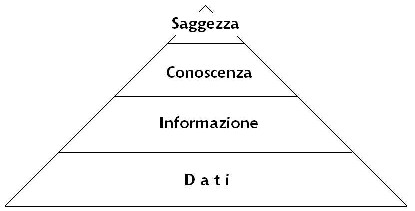
\includegraphics[scale=1.9]{img/piramidepic.png}
	\caption{Schema della gerarchia piramidale del knowledge management}
	\label{fig:piramidepic}
\end{figure}

Come possiamo notare dall'immagine, occorrono diversi raffinamenti prima di arrivare alla conoscenza.
I dati sono materiale grezzo, ovvero numeri e parole relativi a propriet\`a del reale, possono essere sintetizzati ed 
elaborati; in questo modo si ottiene informazione, ovvero dati interpretati, organizzati, contestualizzati e 
oggettivizzati. Infine si passa alla conoscenza, ovvero un insieme dinamico di esperienze concrete, valori,
informazioni ed intuizioni che consente la valutazione e l'inclusione di nuove esperienze ed informazioni.
In altre parole la conoscenza \`e informazione rielaborata ed applicata alla pratica.

\textit {Quindi, qual \`e la sfida per gli informatici?} La sfida consiste nel rappresentare, gestire, 
distribuire e manutenere sia conoscenza codificata che tacita. Questo mediante \textit {l'ingegneria della conoscenza}, 
una disciplina che si occupa dello studio e l'applicazione di metodologie e formalismi per la progettazione e la
realizzazione di \textit {sistemi basati su conoscenza}. 

\begin{section}{Agenti intelligenti}
I sistemi basati su conoscenza sono sistemi artificiali che hanno conoscenza 
del loro obiettivo, del contesto in cui operano e dell'affidabilit\`a della conoscenza su cui operano.
Nel caso in cui utilizzino una rappresentazione esplicita della conoscenza relativa al problema da risolvere,
si parla di \textit{agenti basati su conoscenza}. Questi sono \textit {software che portano a
termine compiti utili}, e sono caratterizzati dell'essere:
\begin{itemize}
    \item \textit {autonomi}, poich\`e l'azione che svolgono \`e guidata da regole e direttive interne;
    \item \textit {reattivi}, in quanto percepiscono aspetti dell'ambiente che li circonda e reagiscono in maniera appropriata;
    \item \textit {proattivi}, poich\`e possono prendere iniziative, intraprendendo azioni in funzione di obiettivi;
    \item \textit {sociali}, in quanto comunicano con altri agenti;
\end{itemize}
Ed \`e proprio grazie a queste caratteristiche \`e possibile parlare di \textit {agenti intelligenti},
dove l'intelligenza \`e descrivibile in termini di conoscenza posseduta dall'agente.
Questi agenti possiedono notevoli livelli di autonomia e agiscono nel loro ambiente in
maniera \textit{soddisfacente, razionale, flessibile}, anche in casi in cui le informazioni
disponibili siano parziali o incerte, esibendo un comportamento intelligente, consapevole, talvolta mostrando
una vera esperienza nel dominio in cui operano.

Esistono diverse applicazioni di questi sistemi: diagnosi e classificazioni, scheduling
di processi produttivi, controllo di robot in situazioni difficili e scarsamente strutturate,
controllo di veicoli autonomi, sistemi cooperativi, filtraggio e categorizzazione di
informazioni presenti sul web e non solo. Tutti questi sistemi apparentemente differenti
hanno molto in comune: un modello dell'ambiente, la possibilit\`a di passare
dall'osservazione all'evidenza, strategie d'azione, apprendimento dalle esperienze passate.
Ma ci\`o che li contraddistingue \`e \textit{la capacit\`a di fare inferenze}, che rende
possibile l'esibizione di un comportamento intelligente. 

L'inferenza \`e un procedimento che a partire da un insieme di \textit{fatti}, ovvero dati
che rappresentano accuratamente specifiche propriet\`a di un dominio, e di \textit{leggi}
(o regole), ovvero regole formali che rappresentano la dinamica del dominio, fa conseguire
nuovi fatti e regole. Per realizzare questa caratteristica \`e necessario un
\textit{meccanismo automatico di inferenza}, o \textit{motore inferenziale}, che si
definisce tramite un meta-interprete della conoscenza, e si realizza in un opportuno linguaggio
(o ambiente) di programmazione.

Quindi affinch\`e una macchina abbia conoscenza e sia in grado di esibire un comportamento intelligente
\`e fondamentale che la conoscenza sia fornita in maniera computabile. Per questo motivo, al fine di costruire
agenti basati su conoscenza \`e necessario definire il dominio, decidere il vocabolario dei predicati, delle variabile
e delle costanti, codificare la conoscenza generale dcondivisa del dominio, codificare una descrizione della 
specifica istanza del problema, e fornire interrogazioni alla procedura di inferenza.   
\end{section}

\begin{section}{Programmazione euristica}
\label{sec:heuristic-programming}
Per realizzare quanto detto finora, la programmazione algoritmica e il modello della macchina di Turing non sono
sufficienti. Viene quindi introdotta la \textit{programmazione euristica}, ramo della computer programming, che fa
uso di \textit{euristiche}, ovvero regole di senso comune derivate dall'esperienza, per risolvere problemi. Tutto ci\`o 
\`e in netto contrasto con la programmazione algoritmica, la quale si basa su procedure matematicamente dimostrabili.
La programmazione euristica invece, permette di definire programmi che risolvono problemi in maniera \textit{automatica}, 
senza un algoritmo definito a priori e tradotto in una sequenza di operazioni da eseguire. Inoltre molti sistemi esperti usano la programmazione euristica.

Nella programmazione euristica l'attenzione si \`e focalizzata, prima che su
metodi e tecniche per rappresentare, manipolare ed elaborarre la conoscenza, su:
\begin{itemize}
	\item \textit{Problem solving}: metodi di per costruire programmi in grado di
    raggiungere obiettivi spesso indeterminati e incerti (per maggiori dettagli si
    veda l'appendice \ref{sec:problem-solving});
	\item \textit{Metodi di ricerca}: metodi che generano tutte le possibili
    soluzioni e le verificano tutte fino a trovarne una adeguata.
\end{itemize}  

Un esempio di problemi che richiedono questo tipo di approccio solutivo sono i giochi
(ad esempio il gioco dell'otto, di cui \`e presente una breve descrizione nell'appendice
\ref{sec:gioco-filetto}), che andrebbero affrontati con metodi \textit{a tentativi};
in questi casi definire una soluzione equivale a ricercare una soluzione nello spazio
dei possibili stati del problema. Quindi \`e necessario rappresentare lo spazio di tutti i
possibili stati del problema, inteso come insieme di tutte le configurazioni possibili,
e va definita l'evoluzione da uno stato ad un altro mediante l'applicazione di operazioni
e regole; vanno inoltre definiti lo stato iniziale e gli stati obiettivo che rappresentano
le possibili soluzioni del problema. Il problema viene risolto mediante la ricerca, ovvero
l'esplorazione dello spazio degli stati per trovare un cammino solutivo, che consenta di
selezionare le appropriate operazioni (o regole) da applicare per arrivare alla soluzione.
\end{section}

\begin{section}{ANT - Another Non-trivial Tool}
ANT, acronimo di \textit{Another Non-trivial Tool}, \`e un tool per lo sviluppo di sistemi basati su conoscenza 
orientato alla risoluzione di giochi. Basato sul modello computazionale dei sistemi di produzione e implementato in C++,
mette a disposizione un linguaggio per la codifica della conoscenza basato sul meccanismo di attivazione delle regole
forward chaining. Nei paragrafi successivi vengono illustrati il modello di calcolo e le motivazioni che ci hanno
portato alla scelta del sopracitato linguaggio.
\end{section}
 
\begin{section}{Modello computazionale}
Il modello computazionale scelto \`e il \textit{il sistema a produzioni} \cite{Jackson99}. Un sistema a
produzioni \`e composto da
\begin{itemize}
    \item una lista ordinata di regole
    \item un interprete di regole che decide quando e quale regola applicare
    \item una memoria di lavoro (working memory), o database globale, che contiene i dati
    che rappresentano lo stato attuale del problema; la working memory viene modificata
    attraverso l'applicazione delle regole.
\end{itemize}

\noindent Le regole di produzione sono della forma:

\begin{figure}[!htb]
	\centering
	
\includegraphics[scale=1.0]{img/formaregole.png}
	\caption{Forma delle regole di produzione}
	\label{fig:formaregole}
\end{figure}

\noindent Nella parte condizione, detta anche \textit{parte sinistra} (LHS, left hand side),
troviamo congiunzioni di letterali booleani che rappresentano l'insieme degli
stimoli percepiti dall'agente; mentre nella parte azione, o \textit{parte destra}
(RHS, right hand side), troviamo le modifiche da apportare all'ambiente
affinch\'e l'ambiente produca nuovi stimoli.  

Il ruolo della working memory \`e di contenere dati nella forma
\textit{attributo-valore}. Questi dati vengono utilizzati dall'interprete per scegliere
quali regole attivare o eseguire in base alla presenza o all'assenza di determinati dati
che soddisfino la condizione di una o pi\`u regole. 

L'interprete per le regole di produzione pu\`o essere descritto in termini di cicli \textit{recognize-act} (riconosci-agisci)
che \`e composto dei seguenti passi:

\begin{itemize}
    \item \textit{matching}: viene verificata la corrispondenza tra la parte sinistra delle regole
          e i dati presenti nella working memory;
    \item \textit{risoluzione dei conflitti}: se ci sono pi\`u regole che possono essere eseguite,
          ne viene scelta una secondo un qualche criterio;
    \item \textit{applicazione della regola}: \`e possibile che venga aggiunto, rimosso o modificato
          un elemento della working memory; dopo questa azione, quindi, si ritorna al passo 1.
\end{itemize}

L'esecuzione si ferma se nessuna regola \`e attiva, oppure se la parte destra di una regola
contiene un comando esplicito per la terminazione. Generalmente, nei sistemi di produzioni,
esistono diverse modalit\`a di attivazione delle regole:
\begin{itemize}
    \item \textit{Forward Chaining} (o concatenazione in avanti): se l'attivazione delle regole
    \`e fatta mediante il matching degli antecedenti con gli elementi della working memory;
    \item \textit{Backward Chaining} (o concatenazione all'indietro): se l'attivazione delle
    regole \`e fatta mediante il matching della parte destra della regola con l'obiettivo che si
    intende raggiungere.
\end{itemize}
\`E interessante notare che il momento di analisi dei dati \`e nettamente separato dal
momento di elaborazione o di modifica dei dati; inoltre alla memoria di lavoro possono
accedere tutte le regole. In aggiunta le regole non ``non chiamano'' altre regole, ma
la connessione degli operatori avviene mediante la memoria di lavoro. \`E altrettanto
importante notare che i sistemi di produzione consentono uno sviluppo incrementale,
ovvero non c'\`e alcun problema nel togliere o aggiungere regole di produzione mantenendo
la coerenza tra di esse (non ambiguit\`a).

Infine \'e possibile individuare un ulteriore classificazione di questi sistemi:
\begin{itemize}
    \item \textbf{Reaction system}: se la parte sconseguente delle regola prevede un'azione;
    \item \textbf{Deduction system}: se la parte sconseguente delle regola prevede una nuova asserzione.
\end{itemize}

	\begin{subsection}{Il problema del matching} 
	Il matching \`e un operazione pesante e strettamente connessa alla complessit\`a della
    rappresentazione del problema; talvolta pu\`o risultare un problema np-completo.
    Questo perch\`e richiede che sia ripetuto su tutte le regole affinch\`e vengano individuate
    tutte le regole applicabili. Ne consegue una ricerca esaustiva tra tutte le regole che
    risulta essere inefficiente e computazionalmente pesante. Quindi il problema richiede
    efficienti algoritmi di matching, in particolar modo per il matching con variabili,
    e la possibilit\`a di ricerca con meccanismi di selezione.

    Inoltre non sempre le precondizioni di una regola sono soddisfatte da un particolare
    stato. Questo tipo di problema \`e poco sentito se le precondizioni vengono definite
    con costanti; diventa invece complesso in presenza di variabili.
	\end{subsection}

	\begin{subsection}{Graph Search}
	Nei sistemi a produzione il problema centrale \`e scegliere una regola applicabile. Una
    caratteristica importante di questa operazione \`e la quantit\`a di conoscenza utilizzata
    nella selezione dalla strategia di controllo. Quindi la ricerca nello spazio degli stati
    pu\`o essere pi\`u o meno informata. Infatti abbiamo:

	\begin{itemize}
	    \item \textit{ricerca cieca}: ricerca sistematica ed esaustiva dello spazio degli
              stati del problema;
	    \item \textit{ricerca informata euristicamente}: ricerca che fa uso di
              conoscenza per ridurre drasticamente lo spazio di ricerca e trovare un cammino ottimale. 
	\end{itemize}

	Generalmente, per realizzare un \textit{meccanismo di inferenza} (o
    interprete di regole) di un sistema a produzioni \`e quello di dotarlo di
    una \textit{graph search} che gli consenta di esplorare lo spazio di ricerca
    per determinare un cammino ottimale. Infatti il problema di trovare una
    sequenza di regole che trasformino un stato del prblema in un altro \`e
    equivalente a trovare un cammino su un grafo orientato in cui ogni nodo
    rappresenta uno stato del problema ed ogni arco una regola che fa passare
    da uno stato ad un altro. Inoltre nella ricerca \`e importante:

	\begin{itemize}
	    \item il modo in cui si rappresentano gli stati del problema, ovvero i
              nodi del grafo su cui organizzare la ricerca;
	    \item la direzione in cui si intraprende la ricerca;
	    \item il modo in cui si selezionano le regole applicabili (efficienza del matching). 	
	\end{itemize}
	\end{subsection}
	  	
	\begin{subsection}{Costi ed efficienza}
	L'efficienza computazionale di un sitema a produzioni dipende da dai costi
    computazionali della strategia di controllo. 
	\begin{figure}[!htb]
	\centering
	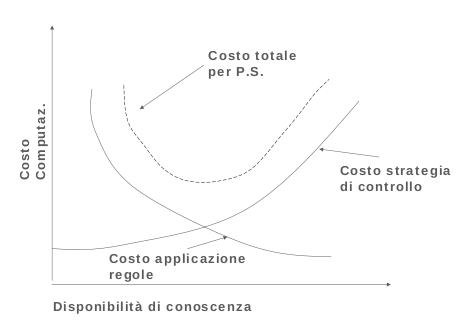
\includegraphics[scale=0.9]{img/costoapplicazioneregole.png}
	\caption{Costo per un production system}
	\label{fig:costoapplicazioneregole}
	\end{figure}
	
	Come possiamo notare dalla figura \ref{fig:costoapplicazioneregole}, i costi dipendono
    dal \textit{costo di applicazione delle regole} e dai \textit{costi di controllo}.
    Inoltre \`e evidente che:

	\begin{itemize}
	    \item ad un estremo, poca conoscenza disponibile implica che la selezione delle
        regole \'e fatta in maniera arbitraria, e quindi un basso costo di controllo
        implica un alto costo di attivazione delle regole;
	    \item all'altro estremo, una conoscenza pi\`u approfondit del problema consente
        di scegliere la regola giusta al momento giusto; quindi alto costo di controllo
        implica basso costo di attivazione delle regole. 	
	\end{itemize}  	
	\end{subsection}
\end{section} 


\begin{section}{Scelta del linguaggio}
ANT \`e scritto in C++. Questa scelta \`e motivata in larga parte dal fatto che
il C++ sia un linguaggio ad oggetti e, come sappiamo, tale paradigma mette a disposizione il concetto 
di astrazione di classe, che ben si presta ad essere considerato per la gestione di un 
sistema di questo tipo. Tuttavia, prima di consacrare il C++ come linguaggio scelto, 
sono stati valutati altri linguaggi come C, Java e Python.

Di fatto, abbiamo scartato subito Java. Nonostante sia un linguaggio orientato
agli oggetti, presenta due notevoli problemi:

\begin{enumerate}
	\item non \`e compilato: questo, in realt\`a, non \`e del tutto vero in quanto
	      Java \`e un linguaggio byte-compilato, ovvero il prodotto del compilatore
				\`e un file che non contiene istruzioni in linguaggio macchina per 
				l'architettura nativa, bens\`i un ``bytecode'' che pu\`o essere
				interpretato solo da una Java Virtual Machine, che per\`o \`e disponibile
				per una moltitudine di piattaforme e, di fatto, rende compatibile lo stesso
				eseguibile per pi\`u sistemi operativi su architetture differenti. Tuttavia
				la JVM aggiunge uno strato di complessit\`a non indifferente dovendo infatti
				traslare le istruzioni dal bytecode al linguaggio macchina. Tralaltro nella
				maggior parte dei casi non c'\`e una corrispondenza uno-ad-uno tra il bytecode
				e il linguaggio macchina (essendo disponibile il processo di traslazione anche per
				architetture diverse dall'x86 usato nei normali calcolatori\footnote{con questa
				espressione intendiamo che l'architettura x86 \`e la pi\`u diffusa nell'ambito
				del personal computing e recentemente ha incrementato la quota di mercato anche
				in ambito server, ma certamente non \`e l'unica: \`e molto probabile, infatti,
				che dispositivi embedded montino processori ARM o Motorola Z80 la cui architettura,
				e quindi anche il rispettivo linguaggio macchina, \`e totalmente diversa da quella
				dell'x86}) pertanto questa operazione non pu\`o, per ovvi motivi, avere tempo costante.
				Negli ultimi anni questo processo ha subito notevoli miglioramenti grazie all'introduzione
				di tecniche di \textit{just in time compilation} \cite{367714} ma, per i
				nostri scopi, questa genere di implementazione \`e un collo di bottiglia non
				indifferente.

	\item la gestione della memoria: in Java la memoria \`e gestita attraverso un
	      processo di \textit{garbage collection}, ovvero l'allocazione e deallocazione
				della memoria \`e una cosa che viene gestita direttamente dalla virtual
				machine tramite l'utilizzo di un sistema di reference counting (ogni oggetto
				che utilizza quella determinata area di memoria incrementa un contatore, che
				viene decrementato non appena l'oggetto in questione non ha pi\`u bisogno di
				utilizzare la memoria allocata; quando questo contatore giunge a zero la
				memoria potr\`a allora essere deallocata) Se per moltissimi ambiti questo
				pu\`o essere solo un vantaggio in quanto riduce la complessit\`a del programma,
				per i nostri scopi questo \`e un problema non indifferente data la grande
				quantit\`a di memoria che viene utilizzata durante l'esecuzione. Inoltre, il
				comportamento della JVM sino alla versione 5, per i nostri scopi, era disastroso
				in termini di performance. Difatti, fino a quella versione, si adottava come
				politica di gestione di garbage collection, quella della non-deallocazione.
				Ovvero la memoria veniva continuamente allocata fino a quando non ce ne era pi\`u
				disponibile. Solo allora veniva invocata la garbage collection che, di fatto,
				bloccava per un certo periodo di tempo l'esecuzione del programma fintanto
				che la memoria non pi\`u utilizzata (ovvero quei blocchi per cui il reference
				counting era giunto a zero) veniva liberata.
\end{enumerate}

Per il Python e il C gli argomenti sono stati meno forti. Rispettivamente, l'impossibilit\`a
di eseguire direttamente il linguaggio macchina per il primo e la mancanza di un pieno
supporto alla programmazione ad oggetti per il secondo, hanno reso di fatto la scelta
del C++ obbligata. In sostanza la scelta del linguaggio si \`e basata su tre punti,
quello della necessit\`a di poter compilare realmente il programma, senza doverlo eseguire
all'interno di macchine virtuali di vario genere, la necessit\`a di dover gestire
manualmente le allocazioni e deallocazioni di memoria e il pieno supporto alla programmazione
ad oggetti.

\end{section}

\begin{section}{Perch\`e ANT?}
Come si \`e gi\`a detto in precedenza, ANT \`e l'acronimo di Another Non-trivial Tool;
\`e abbastanza intuitivo notare la forte contrapposizione tra i termini another (un'altro)
e non-trivial (non banale); infatti ANT \`e solo un altro strumento nel suo genere.
Tuttavia controllare il comportamento di un sistema a regole pu\`o essere un problema non
affatto banale. Citando Peter Jackson \cite{Jackson99}:\\

\quotation{\textit{``Controlling the behaviour of
rule-based systems can pose non-trivial problems''}}
\\

\noindent Ma, tralasciando l'acronimo, \textit{ant} in inglese vuol dire formica,
termine di paragone spesso usato per sottolineare la lentezza di qualcuno o qualcosa;
dando questa seconda accezione, abbiamo voluto esorcizzare il nostro timore riguardo
le prestazioni in termini di velocit\`a della nostra applicazione. 
\end{section}

\begin{section}{Perch\`e un motore inferenziale e non un sistema esperto}
La scelta \`e stata motivata dal fatto che la realizzazione di un motore inferenziale fa
convergere gran parte delle conoscenze acquisite durante tutto il percorso di studi durante
corsi quali quello di ``linguaggi di programmazione'', ``metodi avanzati di programmazione'',
``algoritmi e strutture dati'' ma non solo: teorie sui linguaggi formali, automi, algoritmi,
strutture dati, paradigmi di programmazione, design pattern, architettura dei moderni
calcolatori, matematiche, sono solo alcuni esempi di argomenti la cui utilit\`a
pu\`o essere messa in dubbio durante il corso di studio ma che invece sono addirittura
fondamentali (e non solo necessarie), ed un progetto quale quello da noi scelto ne mette
in risalto le diverse caratteristiche.

La prospettiva di doversi confrontare con problemi reali e complessi sia dal punto di vista
strettamente computazionale che dal punto di vista algoritmico \`e stata un ulteriore
spinta verso la scelta della realizzazione del motore inferenziale piuttosto che il sistema esperto.
\end{section} 

\end{chapter}

\begin{chapter}{Come funziona}

\begin{section}{Schema generale}
ANT \`e diviso in tre componenti logici principali: il \textbf{parser}, la \textbf{
working memory} e gli \textbf{algoritmi}. Ognuno di questi tre componenti
\`e collegato agli altri secondo lo schema seguente:

\begin{figure}[!htb]
	\centering
	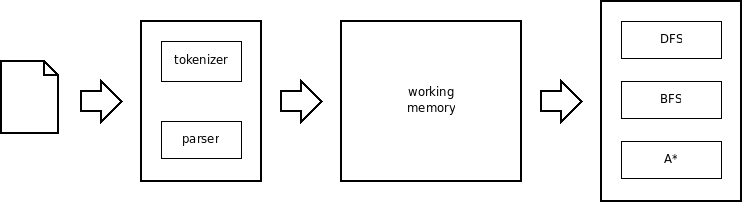
\includegraphics[scale=.45]{img/schemagenerale.png}
	\caption{Schema generale del funzionamento di ANT}
	\label{fig:schemagenerale}
\end{figure}

Si noti che il parser \`e a sua volta diviso in due componenti, il tokenizer
ed il parser vero e proprio, il cui funzionamento verr\`a illustrato in dettaglio
in \ref{sec:parsing-overview}.
La working memory \`e la componente che mantiene in memoria fatti e regole. Verr\`a
descritta in dettaglio in \ref{sec:workingmemory-overview}.
La gestione degli algoritmi verr\`a affrontata, assieme a una descrizione pi\`u
specifica del funzionamento degli stessi, nel capitolo \ref{sec:algoritmi}.

\end{section}

\begin{section}{Grammatica del linguaggio}
Un file sorgente in ANT \`e diviso in quattro componenti principali:
\begin{enumerate}
	\item il blocco delle opzioni
	\item il blocco di fatti
	\item il blocco delle regole
	\item il blocco delle euristiche (opzionale)
\end{enumerate}
\noindent La grammatica completa in notazione BNF \`e disponibile in \ref{sec:grammar}.

	\begin{subsection}{Il blocco delle opzioni}
	\label{sec:option-block}
	Il blocco delle opzioni \`e identificato dalle parole chiave \verb,set, e \verb,endSet, e deve
	essere unico all'interno di tutto il file sorgente
	Ad esempio:

	\begin{verbatim}
	set
	  opzione1 "valore1";
	  opzione2 "valore2";
	  opzione3 3;
	endSet
	\end{verbatim}

	\noindent Le opzioni disponibili sono (obbligatorie a meno che non specificato diversamente):
	\begin{itemize}
		\item \verb,algo,: imposta l'algoritmo da utilizzare per la risoluzione del problema, pu\`o
		essere uno tra \verb,bfs, per la ricerca in ampiezza, \verb,dfs, per la ricerca in profondit\`a,
		\verb,astar, per l'algoritmo A* e \verb,hill, per l'algoritmo di ricerca a salita pi\`u
		ripida (\textit{Hill Climbing})
		\item \verb,limit,: opzionale se l'algoritmo scelto \`e A*, obbligatorio per gli altri algoritmi,
		imposta il limite di profondit\`a per l'algoritmo
		\item \verb,start,: il nome del fatto iniziale
		\item \verb,stop,: il nome del fatto finale
		\item \verb,heuristic,: il nome della funzione euristica, da utilizzare solo se l'algoritmo
		scelto \`e A* oppure quello dell'Hill Climbing
	\end{itemize}
	\end{subsection}

	\begin{subsection}{Il blocco dei fatti}
	Il blocco di un fatto \`e identificato dalle keyword \verb,beginFact, e \verb,endFact,. Ad
	ogni fatto \`e associato un nome di riferimento che deve essere univoco all'interno del
	sorgente. Ogni fatto presenta una lista di attributi che possono assumere valori numerici
	o stringhe. Ad esempio:

	\begin{verbatim}
	beginFact fatto
	  attributo1 = "stringa";
	  attributo2 = 10000;
	  attributo3 = "altra stringa";
	endFact
	\end{verbatim}

	\noindent Non vengono imposti limiti\footnote{sebbene siano presenti, ovviamente, limiti pratici
    sulla quantit\`a di memoria disponibile} sul numero di attributi di un fatto.
	\end{subsection}

	\begin{subsection}{Il blocco delle regole}
	Una regola \`e identificata dalle keyword \verb,beginRule, e \verb,endRule,. Ad
	ogni regola \`e associato un nome di riferimento che deve essere univoco all'interno del
	sorgente. Ogni regola si divide in due parti: LHS (Left Hand Side), parte sinistra, e RHS
	(Right Hand Side), parte destra. Queste due parti sono separate dal carattere \verb,>,.

	La parte sinistra \`e quella che verifica l'applicabilit\`a della regola e non \`e altro
	che un espressione booleana, mentre la parte destra \`e quella che applica modifiche
	alla base di fatti. Le regole possono definire variabili che verranno risolte tramite
	il processo di matching descritto in \ref{sec:matching}. Ad esempio:

	\begin{verbatim}
	beginRule regola
	  equals("attributo", valore) and
	  gt(valore, 3)
	  >
	  remove("attributo");
	endRule
	\end{verbatim}

	\noindent Una lista dei predicati disponibili si trova in \ref{sec:predicates}.
	\end{subsection}

	\begin{subsection}{Il blocco delle euristiche}
    \label{sec:heuristic-block}
    \`E possibile definire, nel caso l'algoritmo specificato lo richieda, una o pi\`u funzioni
    euristiche all'interno di un sorgente. Le euristiche vengono identificate dalle keyword
    \verb,beginHeuristic, e \verb,endHeuristic, che servono rispettivamente a indicare l'inizio di
    una funzione euristica e la sua fine. Ad ogni euristica va associato un nome univoco
    tra le euristiche che verr\`a usato poi per indicare nell'opzione \verb,heuristic,
    (vedi la descrizione delle opzioni disponibili in \ref{sec:option-block})
    quale sar\`a l'euristica da considerare per l'algoritmo (se ha senso considerarla, infatti
    algoritmi quali il BFS e il DFS ignorano la presenza di un euristica).

    Un euristica non \`e altro che una serie di predicati per la parte destra di una regola,
    pertanto i predicati utilizzabili sono esattamente gli stessi definiti per la RHS delle 
    regole (una lista dei predicati \`e disponibile in appendice \ref{sec:predicates-rhs}).

    La vera differenza con la RHS delle regole \`e che, essendo una funzione euristica una
    funzione che ritorna un valore che rappresenta una stima della distanza dallo stato corrente
    all'obiettivo, esiste la necessit\`a di poter \textit{ritornare} il valore in questione.
    Questo viene fatto utilizzando il predicato \verb,return,, il cui unico parametro in
    input \`e il valore di ritorno dell'euristica. \`E possibile avere pi\`u \verb,return,
    all'interno della stessa euristica, ma verr\`a considerato esclusivamente l'ultimo.

    Una semplice euristica di esempio \`e quella utilizzata per il gioco dell'8, dove viene
    contato il numero di tasselli fuoriposto:

    \begin{verbatim}
	beginHeuristic tasselli_mancanti
	  define(h, 0);
	  different("cella_1_1", 1, 1, 1, res);
	  add(h, res);
	  different("cella_1_2", 1, 2, 2, res);
	  add(h, res);
	  different("cella_1_3", 1, 3, 3, res);
	  add(h, res);
	  different("cella_2_1", 2, 1, 8, res);
	  add(h, res);
	  different("cella_2_2", 2, 2, 0, res);
	  add(h, res);
	  different("cella_2_3", 2, 3, 4, res);
	  add(h, res);
	  different("cella_3_1", 3, 1, 7, res);
	  add(h, res);
	  different("cella_3_2", 3, 2, 6, res);
	  add(h, res);
	  different("cella_3_3", 3, 3, 5, res)
	  add(h, res);
	  return(h);
	endHeuristic
    \end{verbatim}

    \noindent In questa euristica, chiamata \verb,tasselli_mancanti,, viene inizializzata una
    variabile \verb,h, che \`e quella che conterr\`a il numero di tasselli fuoriposto. Per
    ogni cella del gioco, se questa non contiene il valore richiesto, viene sommato 1 ad \verb,h,.
    Alla fine \verb,h, sar\`a esattamente il valore che vogliamo far ritornare e pertanto
    procediamo con il \verb,return(h),.

	\end{subsection}

\end{section}

\begin{section}{Il parsing}
\label{sec:parsing-overview}
Il parser \`e diviso in due componenti principali, il tokenizer e il parser vero e
proprio. Il tokenizer si occupa di dividere il file sorgente in token, ovvero separa
i vari \textit{elementi} del file sorgente mentre il parser effettua controlli sulla
validit\`a della sequenza di elementi.

	\begin{subsection}{Tokenizer}
	Come gi\`a detto il tokenizer divide il sorgente in una lista di token che poi
	verranno passati al parser. \`E un automa a stati finiti che non effettua controlli
	di validit\`a semantica, ma semplicemente si assicura che ogni singolo token sia
	in una forma, ovvero di un tipo, accettabile dal programma. Per esempio, sia dato
	il seguente file sorgente:

	\begin{verbatim}
	beginFact nomefatto
	  attributo1 = "valore";
	  attributo2 = 1;
	endFact
	\end{verbatim}

	\noindent Allora verr\`a prodotta la lista seguente:

	\begin{verbatim}
	('beginFact', TKN_SYMBOL), ('nomefatto', TKN_SYMBOL),
	  ('attributo1', TKN_SYMBOL), ('=', TKN_OPERATOR),
	    ('valore', TKN_STRING), (';', TKN_OPERATOR),
	  ('attributo2', TKN_SYMBOL), ('=', TKN_OPERATOR),
	    ('1', TKN_NUMBER), (';', TKN_OPERATOR),
	('endFact', TKN_SYMBOL)
	\end{verbatim}

	\noindent Si pu\`o notare che ogni token e` una coppia valore-tipo. Il tipo pu\`o
	essere un simbolo (\verb,TKN_SYMBOL,), un operatore del linguaggio (\verb,TKN_OPERATOR,)
	o una costante (\verb,TKN_NUMBER, o \verb,TKN_STRING,). Questa lista verr\`a passata
	al parser che proceder\`a a effettuare controlli sulla semantica del sorgente.
	\end{subsection}
	
	\begin{subsection}{Parser}
	Dalla lista ricevuta dal tokenizer, il parser effettua il parsing e vero e proprio
	e inserisce le componenti riconosciute come fatti o regole all'interno delle strutture
	dati apposite. La lista di token viene inizialmente divisa in \textit{blocchi}, ognuno
	relativo ad un elemento del linguaggio come un fatto o una regola. Successivamente,
	ognuno di questi blocchi, viene diviso in sottoblocchi che vengono passati alla routine
	di parsing relativa. Ad esempio, il sorgente viene prima diviso in vari blocchi,
    ognuno specifico di un elemento del programma come il blocco delle opzioni, quello delle
    regole, dei fatti, ecc... A sua volta, ogni blocco viene diviso in sotto-blocchi, ad
    esempio un blocco di tipo fatto viene diviso in modo tale da avere una lista di coppie
    attributo-valore che verr\`a poi parsato dalla routine relativa.
	\end{subsection}
\end{section}

\begin{section}{Avviare ANT}
L'invocazione di ANT avviene tramite command line. \`E possibile passare alcune opzioni
tramite linea di comando, quali:

\begin{itemize}
	\item \verb,--input,: percorso relativo o assoluto verso il sorgente del problema da risolvere;
	\item \verb,--algo,: l'algoritmo da utilizzare. Sovrascrive l'opzione descritta in \ref{sec:option-block};
	\item \verb,--limit,: il limite da imporre sull'algoritmo (il tipo di limite dipende dall'algoritmo e
	in alcuni casi pu\`o non essere considerato). Sovrascrive l'opzione descritta in \ref{sec:option-block};
	\item \verb,--show-stats,: mostra statistiche sull'utilizzo del programma come il numero di nodi
	espansi dall'algoritmo. In ambienti UNIX-like mostra anche statistiche di utilizzo della memoria;
\end{itemize}

Per esempio, il problema dell'agricoltore risolto in \verb,esempi/agricoltore.ant,, si avvia con:

\begin{verbatim}
$ ant --input esempi/agricoltore.ant

ANT v0.77815

Facts in memory: 2
Rules in memory: 8
Processing (algorithm: bfs)...
Limit: 15
Solution found!
Sequence: 
  1. sposta_agricoltore_e_pecora_sulla_riva_lontana
  2. sposta_agricoltore_sulla_riva_vicina
  3. sposta_agricoltore_e_cavolo_sulla_riva_lontana
  4. sposta_agricoltore_e_pecora_sulla_riva_vicina
  5. sposta_agricoltore_e_lupo_sulla_riva_lontana
  6. sposta_agricoltore_sulla_riva_vicina
  7. sposta_agricoltore_e_pecora_sulla_riva_lontana
\end{verbatim}

Se volessimo usare l'algoritmo DFS senza modificare il file sorgente del problema e mostrare le
statistiche di utilizzo, potremmo invece fare:

\begin{verbatim}
$ ant --input esempi/agricoltore.ant --algo dfs --show-stats

ANT v0.77815

Facts in memory: 2
Rules in memory: 8
Processing (algorithm: dfs)...
Limit: 15
Solution found!
Sequence: 
  1. sposta_agricoltore_e_pecora_sulla_riva_lontana
  2. sposta_agricoltore_sulla_riva_vicina
  3. sposta_agricoltore_e_lupo_sulla_riva_lontana
  4. sposta_agricoltore_e_pecora_sulla_riva_vicina
  5. sposta_agricoltore_e_cavolo_sulla_riva_lontana
  6. sposta_agricoltore_sulla_riva_vicina
  7. sposta_agricoltore_e_pecora_sulla_riva_lontana
Usage statistics:
 Expanded nodes:                11
 User time used:                0,11998s
 System time used:              0,2999s
 Page reclaims:                 421
 Page faults:                   1
 No. of swaps:                  0
 Voluntary context switches:    2
 Involuntary context switches:  54
 Total memory used:             3388kB
\end{verbatim}
\end{section}

\begin{section}{La working memory}
\label{sec:workingmemory-overview}
La working memory memorizza una \textit{rappresentazione eseguibile} dei fatti e
delle regole. Sulla working memory viene eseguito il problema, ovvero viene effettuato
il matching (vedi sezione successiva, \ref{sec:matching}) sulle regole disponibili
e tali regole vengono applicate.
\end{section}

\begin{section}{Il problema del matching}
\label{sec:matching}
Il processo di ricerca delle regole applicabili per un determinato stato della working
memory \`e chiamato \textbf{matching}. In particolare, nel momento in cui abbiamo a che
fare con regole che presentano variabili al loro interno, dobbiamo \textbf{unificare}
tali regole con valori che la soddisfano, ovvero dobbiamo trovare una sostituzione delle
variabili tale che la regola risulti applicabile (questo processo \`e chiamato, appunto,
\textbf{unificazione}). Il matching \`e un processo complesso e soprattutto
computazionalmente pesante, pertanto abbiamo dovuto prendere alcuni accorgimenti in fase
di realizzazione.

Il problema \`e stato risolto nel modo seguente. Innanzitutto, le regole sono
divise in due parti logicamente distinte: la parte sinistra o \textit{Left Hand Side}
(LHS) e la parte destra o \textit{Right Hand Side} (RHS).
L'unificazione va risolta esclusivamente sulla parte sinistra; la parte destra
della regola riutilizzer\`a, se necessario, le variabili precedentemente risolte
per la LHS.

All'interno di ANT, la parte sinistra non \`e altro che un albero di espressione, ovvero
un albero binario le cui foglie sono nodi di tipo predicato, mentre le radici sono
nodi che rappresentano un espressione booleana (``and'' oppure ``or''). In questo modo
\`e possibile valutare l'albero ricorsivamente attraverso le visite canoniche quali
quelle in preordine, postordine o in ordine a seconda delle necessit\`a.

Nel caso la regola non presenti variabili, percui non sia necessario unificare, allora
viene semplicemente valutato l'albero di espressione sullo stato corrente.

L'algoritmo di unificazione implementato da ANT funziona secondo lo schema seguente.
Per ogni regola presa in esame:

\begin{enumerate}
	\item estrai una coda di predicati attraverso una visita in post-ordine
	      dell'albero di espressione
	\item dalla coda precedentemente creata, estrai una lista di variabili
	      e informazioni sul loro tipo
	\item esplora tutto lo spazio di ricerca creando un albero n-ario a partire
        dalle variabili estratte e provando, in sostanza, tutte le possibili
        combinazioni
	\item valuta la regola per ogni possibile sostituzione e aggiungi al
        conflict set solo le regole la cui LHS ritorna il valore di verit\`a "vero"
\end{enumerate}

Il cuore del problema \`e il punto tre: la creazione e gestione dell'albero pu\`o
essere un problema rilevante dato la grande quantit\`a di nodi presenti. Inizialmente
avevamo utilizzato un heap per gestire l'albero \cite{Skiena08}.
Questa scelta, fatta per ridurre il consumo di memoria essendo l'heap in sostanza un'area
contigua di memoria, \`e risultata subito inapplicabile.
Difatti, l'heap non \`e altro che un array di dimensione prefissata il cui generico
elemento alla posizione \verb,k,, in un albero \verb,n,-ario ha:

\begin{itemize}
	\item genitore in posizione $\lfloor\frac{1}{n}(k-1)\rfloor$
	\item figlio i-esimo in posizione $nk+i$, $1 \leq i \leq n$
\end{itemize}

\noindent(Nel caso di un albero binario, la formula per ottenere i figli destro e sinistro
si riduce a $2k+1$ per il figlio sinistro e $2k+2$ per il figlio destro)

La scelta dell'heap porta una serie di miglioramenti nelle prestazioni rispetto
all'utilizzo di un canonico albero n-ario con puntatori, ed \`e giustificata
dal fatto che l'albero di espressione \`e perfettamente bilanciato, pertanto
l'array non sar\`a sparso e, anzi, tutti i campi saranno utilizzati. Inoltre,
dato che i nodi sono tutti presenti in una sezione di memoria contigua (esattamente
quella occupata dall'array su cui l'heap \`e implementato), sfruttiamo la cache
del processore in due modi:

\begin{itemize}
	\item nei processori moderni la cache pu\`o variare da un minimo
          di 512k fino anche a 8Mb sui processori per server. Nel caso in cui l'albero sia
          relativamente piccolo, potremo inserirlo tutto nella cache evitando,
          quindi l'accesso alla memoria centrale con conseguente risparmio di tempo
	\item usiamo la cache line: sui moderni processori la cache line \`e una tecnica
          che ci assicura di inserire nella cache, nel momento in cui richiediamo l'accesso
          ad un dato indirizzo di memoria, un intero blocco di memoria contenente
          l'indirizzo richiesto. Questo blocco ha dimensione fissa, appunto la
          \textit{cache line} che ha grandezza variabile a seconda delle implementazioni.
          Nei processori comuni la cache line \`e grande 64 bytes ma in realt\`a
          pu\`o variare da un minimo di 8 a un massimo di 512 bytes a seconda dell'architettura
          del processore.
\end{itemize}

Come gi\`a detto, l'heap \`e risultato tuttavia inapplicabile. La motivazione risiede
nel fatto che il numero di nodi, che \`e noto a priori, \`e estremamente elevato. Inoltre,
l'heap richiede che la memoria allocata sia contigua e sia disponibile un accesso diretto
(percui la scelta dell'array). Questo ci permette di ridurre la memoria usata dai puntatori,
ma in compenso abbiamo bisogno di allocare in blocco tutta la memoria richiesta.
Consideriamo, ad esempio, il caso in cui abbiamo cinque variabili che possono assumere venti
valori. Il nostro albero sar\`a quindi un albero di grado venti e di profondit\`a cinque.
Supponiamo che ogni nodo occupi 10 bytes, allora, essendo l'albero bilanciato (ma
utilizzando un heap anche se non utilizziamo alcuni nodi questi vanno comunque allocati),
avremo bisogno di $\sum_{i=1}^5{(20^i \cdot 10)} = 67368200$ bytes, ovvero circa 65Mb.

\`E facile capire come al crescere del numero delle variabili e all'aumentare dei valori che
queste possono assumere, l'heap raggiunge presto una dimensione eccessiva. Abbiamo, quindi,
dovuto trovare una soluzione alternativa che ci permettesse comunque di risolvere velocemente,
per quanto possibile, il problema dell'unificazione. Alla fine, la scelta \`e ricaduta
su due \textit{semplici} vettori di elementi. Infatti, si pu\`o notare un pattern all'interno
di questo processo. Ovvero, una volta calcolati, i valori che le variabili possono assumere
sono sempre gli stessi indipendentemente dalla profondit\`a dell'albero (e, quindi, dalla
variabile che stiamo considerando).

Si considerano due vettori: uno terr\`a in memoria i valori che le variabili possono assumere
(chiameremo questo vettore \verb,VALUES, in seguito), l'altro invece sar\`a un vettore di
tanti elementi quanti sono le variabili (questo vettore lo chiameremo \verb,VAR,).
\verb,VAR, non fa altro che tenere in memoria a quale indice la variabile di posizione \verb,x,
punta su \verb,VALUES,. Inizialmente tutti gli elementi di \verb,VALUES, puntano al primo
elemento di \verb,VAR,. Viene quindi valutata l'espressione, con le variabili risolte
secondo l'elemento a cui esse puntano su \verb,VALUES, e in caso di successo la sostituzione
effettuata, assieme alla regola a cui essa \`e associata, viene aggiunta al conflict set.
Si incrementa quindi il valore dell'ultimo elemento di \verb,VAR, e si ripete la procedura
di valutazione. Quando questo valore raggiunge la dimensione di \verb,VALUES,, questo
viene riportato a zero e viene incrementato l'indice a cui punta la variabile seguente.
In questo modo abbiamo comunque esplorato tutto lo spazio di ricerca, ma abbiamo utilizzato
pochissima memoria rispetto all'heap. Difatti, se supponiamo che dieci variabili possono
assumere 30 possibili valori, avremo soltanto due vettori rispettivamente da 10 e 30 elementi.

\noindent Prendiamo in esame la regola che segue per capire meglio come viene
risolto il processo di unificazione:

\begin{verbatim}
beginRule
  equals(attributo1, attributo2) and
  gt(attributo2, 3)
  >
  ...
endRule
\end{verbatim}

Espressa in linguaggio naturale, la regola verr\`a soddisfatta quando ``esistono due
attributi all'interno del fatto, percui uno sia maggiore di tre e l'altro sia uguale
al primo (pertanto, anch'esso sar\`a maggiore di tre)''. Notiamo che, implicitamente,
si \`e applicato un meccanismo di inferenza sulla regola. Questo \`e un comportamento
classico nei sistemi di questo tipo.

\begin{figure}[!htb]
	\centering
	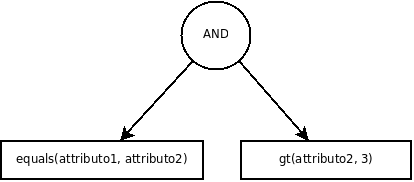
\includegraphics[scale=.45]{img/alberoregolasemplice.png}
	\caption{Albero di espressione per una regola semplice}
	\label{fig:alberoregolasemplice}
\end{figure}

Una volta costruito l'albero, ha luogo il processo di unificazione. Innanzitutto,
viene estratta dal fatto in esame una lista di attributi-valore e, successivamente,
viene creato un secondo albero (in ANT \`e implementato tramite i due vettori descritti
sopra) come in figura \ref{fig:alberounificazione}.

\begin{figure}
	\centering
	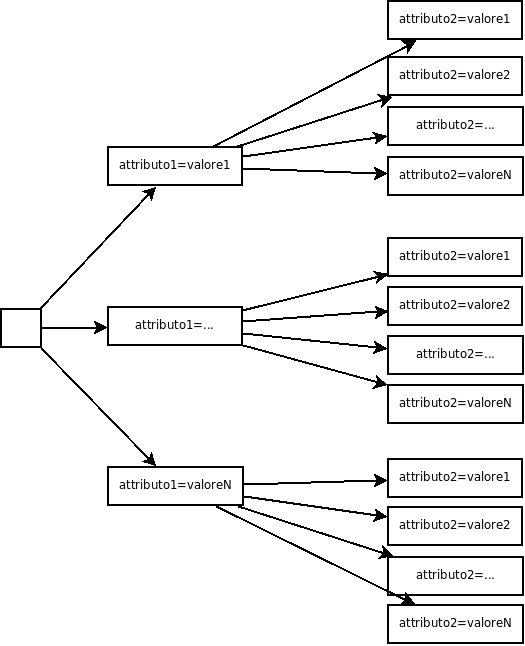
\includegraphics[scale=.45]{img/alberounificazione.png}
	\caption{Albero di unificazione}
	\label{fig:alberounificazione}
\end{figure}

Come si pu\`o notare, ogni variabile presente nella regola in esame viene
``sostituita'' con un possibile valore all'interno degli attributi del
fatto. La valutazione dell'espressione viene effettuata nel momento in si
\`e raggiunta una foglia dell'albero, e le variabili vengono sostituite
con i valori precedentemente ritrovati. Se la valutazione \`e positiva,
ovvero la regola \`e applicabile, allora tale regola assieme alle
corrispondenze variabili-valori trovate, viene aggiunta al conflict set.

Si noti che per una stessa regola possono esserci pi\`u sostituzioni valide.
Per esempio, consideriamo la seguente situazione:

\begin{verbatim}
beginFact fatto
  a = 1;
  b = 2;
  c = 3;
endFact

beginRule regola
  gte(attributo, 1)
  >
  ...
endRule
\end{verbatim}

In questo caso la regola potr\`a attivarsi tre volte con tre con differenti
sostituzioni, ovvero \verb,<attributo=1>,, \verb,<attributo=2>,, \verb,<attributo=3>,,
percui al conflict set verranno aggiunte tre diverse attivazioni che condividono la
struttura della regola ma non i valori su cui essa si applica.
\end{section}

\begin{section}{Applicazione dell'algoritmo scelto}
Indipendentemente dall'algoritmo specificato tramite l'opzione \verb,algo, oppure
quello richiesto dall'opzione \verb,--algo, per la command line, si procede in modo
simile per tutti gli algoritmi. \`E difatti possibile definire un nuovo algoritmo
senza grossi problemi, quello che \`e richiesto \`e che la funzione da richiamare
abbia la seguente firma:

\begin{verbatim}
uint32_t(*AlgoRunner)(RuleSet *ruleset,
                      Fact *initial,
                      Fact *final,
                      Options *options)
\end{verbatim}

\noindent (Il tipo di dati \verb,uint32_t, definisce un intero senza segno di 32 bit,
rimanendo per\`o indipendente dall'architettura sottostante. Questo permette di
garantire che gli interi abbiano sempre 32 bit indipendentemente dall'architettura
utilizzata, che sia x86 o ARM o Z80)\\

\noindent Ovvero, dev'essere una funzione che prende come parametri di input
un \verb,ruleset, ovvero la lista di tutte le regole presenti nel programma,
la coppia di fatti \verb,initial, e \verb,final, che rappresentano rispettivamente il
fatto da cui si parte per la computazione e il fatto a cui vogliamo arrivare ed una
lista di opzioni, ovvero tutte le opzioni definite sia tramite il blocco delle
opzioni che tramite command line (\`e sostanzialmente un dizionario le cui chiavi
sono i valori delle opzioni descritte in \ref{sec:option-block}).
\end{section}

\end{chapter}

\begin{chapter}{Algoritmi disponibili}
\label{sec:algoritmi}

In ANT sono stati implementati due tipi di algoritmi di ricerca:
\begin{itemize}
	\item Ricerca non informata (o a \textit{tentativi} o anche \textit{cieca})
	\item Ricerca informata
\end{itemize}

Queste due tipologie di ricerca differiscono per la presenza, nella ricerca
informata, di una \textbf{funzione euristica} che non fa altro che fornire una
stima della distanza dall'obiettivo tramite una rappresentazione matematica della
conoscenza del problema. Per esempio, nel problema classico del gioco dell'otto,
la nostra funzione euristica potrebbe essere una funzione che conta il numero di
caselle fuoriposto rispetto alla configurazione finale. Tale funzione \`e quella
descritta durante la descrizione del blocco delle euristiche in \ref{sec:heuristic-block}.
Analizzeremo, comunque, questo caso pi\`u nello specifico in \ref{sec:heuristicdef}.

La scelta di un algoritmo rispetto ad un altro e, intrinsecamente, lo studio
dell'algoritmo in s\'e per s\'e si basa su quattro fattori:

\begin{enumerate}
	\item \textbf{completezza}: la garanzia di trovare una soluzione valida per
        il problema in esame, se esiste
	\item \textbf{complessit\`a temporale}: il tempo richiesto dall'algoritmo per
        risolvere il problema
	\item \textbf{complessit\`a spaziale}: la quantit\`a di memoria richiesta
        dall'algoritmo per risolvere il problema
  \item \textbf{ottimalit\`a}: la garanzia di trovare la soluzione \textit{ottima}
        nel caso esistano pi\`u soluzioni per lo stesso problema (es: trovare il
        percorso minimo tra due citt\`a),
\end{enumerate}

Gli algoritmi implementati mostrano diverse caratteristiche per ognuno di questi
fattori. Per i dettagli relativi a completezza, complessit\`a temporale e spaziale
e ottimalit\`a di ogni singolo algoritmo si rimanda a \cite{norvig03} che fornisce
una discussione approfondita sia dell'algoritmo in s\'e per s\'e che un'analisi di
tutti i fattori sopra descritti relativamente all'algoritmo in questione.

I metodi di ricerca non informati si basano sulla possibilit\`a di esplorazione
dell'intero spazio di ricerca. Come \`e facile intuire, spesso l'ampiezza dello
spazio di ricerca \`e estremamente ampia e questi algoritmi risultano inapplicabili
sia in termini di complessit\`a temporale che spaziale.

Per velocizzare l'applicazione degli algoritmi ed evitare l'ingresso in cammini
ciclici (ovvero da un nodo si genera il suo genitore, quindi si ripete il ciclo
all'infinito) oppure gi\`a considerati, durante la generazione di ogni nuovo nodo
nell'albero di ricerca viene controllato se il nodo in questione \`e stato gi\`a
generato. Questa verifica \`e fatta creando, per ogni nodo generato, un hash della
sua rappresentazione ed inserendo tale rappresentazione in un \verb,set,. In questo
modo, la ricerca di un hash precedentemente calcolato ha complessit\`a $O(1)$.

La discussione dei due algoritmi di ricerca non informata implementati, ovvero
ricerca in ampiezza (\textit{Breadth First Search} o \textit{BFS}) e ricerca in
profondit\`a (\textit{Depth First Search} o \textit{DFS}) segue rispettivamente
in \ref{sec:non-informed-algos} mentre i due algoritmi di ricerca informata A* e
Hill climbing sono discussi in \ref{sec:informed-algos}.

Nei capitoli che seguono, il problema di riferimento \`e quello del gioco dell'8
che viene illustrato in appendice \ref{sec:gioco-filetto}.

\begin{section}{Algoritmi di ricerca non informata}
\label{sec:non-informed-algos}
Come gi\`a detto in precedenza, gli algoritmi di ricerca non informati si basano
sulla possibilit\`a di esplorare l'intero spazio di ricerca. Questo, per\`o, potrebbe
non essere sempre possibile per diversi motivi:

\begin{itemize}
    \item lo spazio di ricerca \`e particolarmente ampio: potrebbe succedere che
    il problema in questione ha uno spazio di ricerca troppo grande per essere
    totalmente esplorato. Il gioco dell'8 ne \`e un esempio, difatti teoricamente
    l'albero ha profondit\`a infinita essendo possibile spostare il tassello e poi
    riportarlo nella sua posizione precedente e continuando cos\`i all'infinito.
    Questo problema pu\`o essere minimizzato evitando le ripetizioni di stati,
    evitando di fatto di ripercorrere cammini gi\`a analizzati.
    \item non abbiamo la certezza che la soluzione esista: questo significa che
    potrebbe succedere di esplorare tutto lo spazio di ricerca senza per\`o
    arrivare ad uno stato finale per il problema in questione (questo non \`e
    valido per il gioco dell'8 in quanto, se la configurazione di partenza \`e
    una configurazione valida, allora sicuramente questa porter\`a ad uno stato
    finale accettabile).
\end{itemize}

In ANT \`e possibile definire un limite tramite la clausola \verb,limit, descritta in
\ref{sec:option-block} che impone un limite sulla profondit\`a raggiungibile dall'albero
delle soluzioni. In questo modo, tutte le configurazioni con una profondit\`a maggiore o
uguale del limite imposto verranno ignorate. Tale limite si dimostra particolarmente
utile durante l'applicazione del DFS.

	\begin{subsection}{Breadth-First search}
    Il \textit{Breadth-First search} o \textit{BFS} effettua una ricerca in ampiezza
    sull'albero delle soluzioni. Partendo dalla configurazione iniziale (livello 0 o radice),
    genera tutte le possibili configurazioni successive (livello 1). Dopodich\'e
    per ogni nodo del livello 1, genera tutte le sue configurazioni successive (livello
    2) e cos\`i via sino a quando viene riconosciuta una configurazione finale
    valida oppure non \`e possibile continuare, ossia non ci sono altre configurazioni
    generabili oppure tutte quelle generabili sono state gi\`a percorse.

    Questo modo di procedere ci assicura che se almeno una soluzione esiste, verr\`a
    trovata, ed in particolar modo verr\`a trovata quella col il cammino pi\`u breve.

    \begin{figure}[!htb]
        \centering
        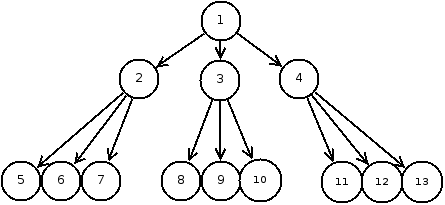
\includegraphics[scale=0.5]{img/bfs.png}
        \caption{Ordine di espansione dei nodi nel BFS}
        \label{fig:bfs-tree}
    \end{figure}

    Bisogna tuttavia notare che questo algoritmo \`e applicabile nel caso in cui il
    grafo, che nel nostro caso \`e implicito, non sia pesato. Questo \`e sempre vero
    nel nostro caso, dato che assumiamo che la generazione di un nuovo nodo non abbia
    peso (in realt\`a questa \`e un'assunzione che facciamo solo nel caso degli algoritmi
    non informati). Nel caso si disponga di un grafo pesato, \`e possibile utilizzare
    algoritmi pi\`u complessi come quello per la ricerca del cammino minimo in un grafo
    di Dijkstra \cite{Skiena08}.

    L'applicazione di questo algoritmo ha senso per determinate istanze del gioco dell'8,
    in quanto le configurazioni generabili da ogni nodo possono essere al massimo quattro
    nel caso in cui il tassello vuoto si trovi al centro del quadrato di gioco, potendosi
    quindi muovere in su, in gi\`u, a destra ed a sinistra. Inoltre, la profondit\`a
    dell'albero da generare dipende dal numero di mosse minime richieste per risolvere la
    particolare istanza del problema. Un'istanza che richiede un minimo di cinque mosse per
    raggiungere la configurazione finale avr\`a difatti un albero di profondit\`a cinque. 
    Dunque, se la profondit\`a dell'albero \`e limitata, cio\'e il gioco \`e risolvibile
    in poche mosse, allora il BFS \`e un algoritmo accettabile\footnote{per accettabile si
    intende computazionalmente possibile in termini di tempo/risorse necessarie per risolvere
    il gioco.} per il gioco dell'8.
	\end{subsection}

	\begin{subsection}{Depth-First search}
    Il \textit{Depth-First search} o \textit{DFS}, al contrario del BFS, effettua una
    ricerca in profondit\`a sull'albero delle soluzioni. Ci\`o significa che, partendo
    dalla configurazione iniziale (livello 0 o radice), genera tutte le possibili
    configurazioni successive. Dopodich\'e prende il primo figlio generato e lo
    considera come una nuova radice e ripete l'operazione. Questo porta ad esplorare
    tutti i cammini che passano da una determinata configurazione, fermandosi solo quando
    si raggiunge una configurazione finale valida oppure non ci sono pi\`u nodi generabili.
    Nel caso si dovessero verificare una delle due condizioni ora citate si ritorna al
    nodo genitore e si procede con l'esplorazione di un cammino alternativo.

    \begin{figure}[!htb]
        \centering
        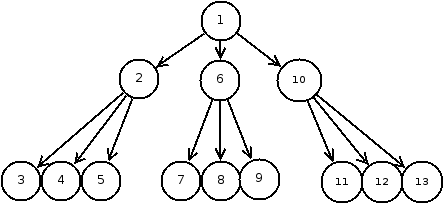
\includegraphics[scale=0.5]{img/dfs.png}
        \caption{Ordine di espansione dei nodi nel DFS}
        \label{fig:dfs-tree}
    \end{figure}
	\end{subsection}

    Il DFS non da nessuna garanzia sul ritrovamento di una soluzione ottima n\'e
    ottimale, ma ci garantisce che, se almeno una soluzione esiste, sar\`a trovata.
    \`E possibile infatti che il DFS trovi una soluzione qualunque piuttosto che
    trovare la soluzione ottima (cosa che non succede, invece, col BFS).

    L'utilizzo del DFS \`e utile nei casi in cui la profondit\`a dell'albero generato
    non sia eccessiva, ossia in problemi in cui siano possibili un numero limitato
    di \textit{mosse} a partire da ogni determinata configurazione. A prova di ci\`o
    si segnala l'inadeguatezza del DFS per il gioco dell'8, comprovata dalle tabelle
    in \ref{tbl:confronto-algoritmi}. In questo specifico problema, per ogni configurazione,
    sono disponibili sempre almeno due mosse\footnote{a meno che queste due mosse non
    portino a configurazioni gi\`a generate in precedenza e che quindi non avrebbe senso
    ripetere}, pertanto ogni nodo pu\`o generare sempre, con le dovute considerazioni,
    almeno due ulteriori cammini.
\end{section}

\begin{section}{Algoritmi di ricerca informata}
\label{sec:informed-algos}

Gli algoritmi di ricerca informata si basano sulla disponibilit\`a di una \textit{funzione
euristica}, ovvero di una funzione matematica in grado di fornire una stima della distanza
di una particolare configurazione dall'obiettivo.
La presenza di tale funzione permette a questo genere di algoritmi di risolvere alcuni
problemi senza aver bisogno di esplorare tutto lo spazio di ricerca che, come gi\`a affermato
pi\`u volte, pu\`o essere talmente ampio da rendere praticamente impossibile, dal punto vista
di risorse necessarie, la sua totale esplorazione. Per una spiegazione dettagliata
sull'utilit\`a delle funzioni euristiche e sulla loro ammissibilit\`a (in semplici parole, un
euristica ammissibile non sbaglia mai per eccesso la stima del costo per raggiungere
l'obiettivo) si rimanda a \cite{norvig03}.

    \begin{subsection}{Definizione della funzione euristica}
    \label{sec:heuristicdef}
    Una funzione euristica deve fornire una stima, in termini numerici, della distanza
    dall'obiettivo. Chiaramente ci\`o dipende dal problema in oggetto, pertanto ANT mette a
    disposizione la possibilit\`a di definire una o pi\`u funzioni euristiche.
    Una funzione euristica in ANT si definisce tramite il blocco \verb,beginHeuristic,-\verb,endHeuristic,
    di cui si pu\`o trovare una descrizione formale in \ref{sec:heuristic-block}.

    Ad esempio per il gioco dell'otto abbiamo individuato due possibili funzioni euristiche:
    \begin{itemize}
        \item una funzione semplice che consiste nel contare il numero di tasselli non in
        posizione corretta. L'idea alla base \`e che tanti pi\`u tasselli saranno fuori posto
        tanto pi\`u distante sar\`a l'obiettivo.
        Sia $pos(x, C)$ la funzione che ritorna $1$ se il tassello $x$ non \`e in posizione corretta
        per la configurazione $C$ e $0$ altrimenti, allora la funzione euristica sar\`a definita come
        $h(n, C) = \sum_{i=1}^{8}{pos(i, C)}$ ove $n$ \`e il nodo che stiamo considerando. Ad esempio,
        per la seguente configurazione il valore ritornato dalla funzione euristica sar\`a $4$.

        \begin{center}
        \begin{tabular}{| c | c | c |}
        \hline
        8 & 1 & 3\\\hline
        7 &   & 4\\\hline
        6 & 2 & 5\\\hline
        \end{tabular}
        \end{center}

        \item la distanza di Manhattan, che consiste nel sommare, per ogni tassello, il numero
        di operazioni necessarie per portarlo in posizione corretta. Come si pu\`o intuire,
        questa funzione consente una valutazione molto pi\`u precisa di quella dei
        tasselli mancanti. Per la stessa configurazione vista precedentemente, la distanza di
        Manhattan sar\`a $5$.
    \end{itemize}

    Si pu\`o notare che i valori ritornati dalle due euristiche, a parit\`a di configurazione,
    sono diversi. In particolare, la distanza di Manhattan considera la stessa configurazione
    pi\`u \textit{lontana} dall'obiettivo rispetto all'euristica dei tasselli fuori posto.
    \end{subsection}

    \begin{subsection}{A*}
    Sia $g(n)$ la funzione che ritorna il costo del cammino dal nodo iniziale al nodo $n$ (in ANT
    tale valore \`e l'indice della profondit\`a del nodo, ovvero il numero di nodi da attraversare
    a partire dalla radice per raggiungere il nodo $n$) ed $h(n)$ la funzione euristica per il
    problema in questione, allora la funzione $f(n) = g(n) + h(n)$ fornir\`a una valutazione della
    distanza del nodo su cui viene applicata dall'obiettivo.

    Per ogni nodo dell'albero delle soluzioni, A* genera tutti i suoi possibili successori applicando
    la $f(n)$ su di essi e memorizzandone il valore risultante come costo associato per raggiungere
    l'obiettivo. Tali nodi vengono inseriti in una coda con priorit\`a ordinata in base al costo
    precedentemente calcolato; allora il successivo nodo da espandere sar\`a l'elemento in cima alla
    coda con priorit\`a.

    Una volta raggiunto l'obiettivo, si procede a ritroso verso il nodo radice per individuare il
    cammino seguito. Tale cammino sar\`a non solo una soluzione del problema, sar\`a anche la
    soluzione ottima. Questo \`e provato dal requisito di ammissibilit\`a della funzione euristica
    introdotto nei capitoli precedenti. La dimostrazione di tale affermazione \`e riportata
    in \cite{norvig03}.
    \end{subsection}

    \begin{subsection}{Hill Climbing}
    L'idea alla base dell'hill climbing \`e quella di seguire sempre il percorso pi\`u promettente.
    Come in A*, quando vengono generati i successori per ogni nodo, viene calcolato il costo
    stimato per raggiungere l'obiettivo tramite la funzione $f(n)$ vista nel capitolo precedente.
    A differenza dell'A* i nodi non vengono inseriti in una coda con priorit\`a, bens\`i viene
    preso il nodo con il costo minore ignorando gli eventuali altri nodi.

    \begin{figure}[!htb]
        \centering
        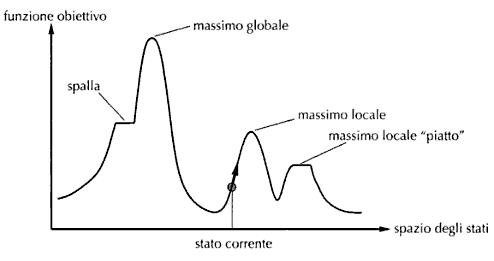
\includegraphics[scale=0.5]{img/hillclimbing.png}
        \caption{Rappresentazione grafica dell'algoritmo di Hill Climbing, fonte \cite{norvig03}}
        \label{fig:hillclimbing}
    \end{figure}

    Si immagina la scalata di una montagna dove, idealmente, la strada pi\`u ripida tra quelle vicine
    \`e quella che permette di raggiungere in minor tempo la cima (obiettivo). Questo pu\`o portare
    alcuni problemi come quelli in figura:
    \begin{itemize}
        \item raggiungendo la \textit{spalla}, sia a destra che a sinistra della posizione corrente
        non si ha n\'e una salita n\'e una discesa. Si pone quindi il problema di dover scegliere
        una delle due direzioni senza avere indicazioni su quale strada sia meglio seguire.
        \item esiste il rischio di raggiungere un \textit{massimo locale}, ovvero si \`e raggiunta
        una cima che per\`o non \`e la soluzione del problema. Sia a destra che a sinistra sono
        presenti strade in discesa che pertanto non vengono considerate.
    \end{itemize}

    \`E possibile evitare questi problemi utilizzando procedure di backtracking nel caso in cui si
    raggiungesse una situazione di stallo, ma nella nostra implementazione abbiamo utilizzato la
    versione nai\"ve dell'algoritmo in cui non prendiamo in considerazione questi problemi. Difatti,
    come si pu\`o vedere in \ref{tbl:confronto-algoritmi-2}, l'algoritmo di hill climbing non
    riesce a trovare una soluzione per il problema del gioco dell'8 al contrario degli altri
    algoritmi.
    \end{subsection}
\end{section}

\begin{section}{Confronto tra gli algoritmi}
Abbiamo scelto un problema classico non banale quale quello del gioco dell'8
e abbiamo messo a confronto i diversi algoritmi descritti nelle sezioni
precedenti. I risultati ottenuti rispettano appieno le nostre aspettative,
difatti gli algoritmi informati si sono dimostrati molto pi\`u veloci di
quelli non informati. Tuttavia, su una piccola istanza del problema (gioco
dell'8 risolvibile in due mosse) gli algoritmi hanno avuto pi\`u o meno
le stesse performance. Questo \`e dovuto al fatto che l'albero di ricerca
in questo caso \`e molto piccolo, pertanto la sua completa esplorazione non
richiede un tempo eccessivo.

\noindent Nella tabella che segue, sono riassunti i risultati che abbiamo ottenuto:

\label{tbl:confronto-algoritmi}

\begin{center}
    \label{tbl:confronto-algoritmi-1}
    \begin{tabular}{| c | c | c | c | c | c |}
    \hline
    \multicolumn{6}{|c|}{\textit{Gioco dell'8 risolvibile in due mosse}} \\
    \hline
                     & A* (1) & A* (2) & Hill climbing & BFS    & DFS     \\\hline
    Tempo di         &        &        &               &        &         \\
    esecuzione       & 0.716s & 0.732s & 1.232s        & 0.808s & 27.421s \\\hline
    Mosse            &        &        &               &        &         \\
    richieste        & 2      & 2      & 2             & 2      & 10      \\\hline
    Memoria          &        &        &               &        &         \\
    occupata         & 3280Kb & 3280Kb & 3280Kb        & 3280Kb & 3664Kb  \\\hline
    Nodi espansi     & 3      & 3      & 2             & 2      & 254     \\\hline
    Limite           &        &        &               &        &         \\
    (se applicabile) & n/a    & n/a    & 10            & 10     & 10      \\\hline
    \end{tabular}
\end{center}

\noindent \\Le due diverse esecuzioni di A* si riferiscono alle due euristiche
descritte in precedenza, in particolare la (1) si riferisce all'euristica della
distanza di Manhattan mentre la (2) si riferisce all'euristica del conteggio dei
tasselli fuoriposto.

Nel confronto successivo \`e stata utilizzata un'istanza del problema pi\`u
complessa per evidenziare le diverse caratteristiche degli algoritmi.
Difatti, nel caso seguente, sono richieste almeno sette mosse per risolvere il problema:

\begin{center}
    \label{tbl:confronto-algoritmi-2}
    \begin{tabular}{| c | c | c | c | c | c |}
    \hline
    \multicolumn{6}{|c|}{\textit{Gioco dell'8 risolvibile in sette mosse}} \\
    \hline
                     & A* (1) & A* (2) & Hill climbing & BFS     & DFS      \\\hline
    Tempo di         &        &        &               &         &          \\
    esecuzione       & 1.956s & 5.963s & 7.244s        & 13.548s & 115.411s \\\hline
    Mosse            &        &        &               &         &          \\
    richieste        & 7      & 7      & n/a           & 7       & 9        \\\hline
    Memoria          &        &        &               &         &          \\
    occupata         & 3280Kb & 3408Kb & 3408Kb        & 3536Kb  & 4944Kb   \\\hline
    Nodi espansi     & 26     & 78     & 21            & 131     & 1167     \\\hline
    Limite           &        &        &               &         &          \\
    (se applicabile) & n/a    & n/a    & 10            & 10      & 12       \\\hline
    \end{tabular}
\end{center}

\noindent \\ Come nel caso precedente, i due A* si riferiscono rispettivamente al
caso in cui viene utilizzata l'euristica della distanza di Manhattan e quello in
cui l'euristica \`e quella del conteggio dei tasselli fuoriposto. Bisogna notare
che l'algoritmo di hill climbing in questo caso non ha saputo trovare una soluzione
al problema.

\end{section}

\end{chapter}

\begin{chapter}{Conclusioni}

\begin{section}{Performabilit\`a delle strutture dati}
Per alcuni problemi sono state testate diverse implementazioni di strutture dati
che hanno prodotto risultati sostanzialmente diversi. Innanzitutto, come gi\`a
descritto in \ref{sec:matching}, per risolvere il problema del matching
abbiamo provato ad utilizzare un albero n-ario canonico. Questo ha portato
enormi problemi durante la risoluzione del problema dell'unificazione in quanto
la creazione, nonch\'e l'accesso e la ricerca dei nodi, era troppo lenta per
i nostri scopi. Si \`e quindi deciso di provare ad utilizzare un heap (vedi
\ref{sec:matching}) ma allora ci si \`e accorti che la memoria richiesta
era semplicemente troppa (ricordiamo che, inoltre, l'heap richiede che sia
allocabile una sezione contigua di memoria). Si \`e allora scelto di utilizzare
la struttura dati \textit{banale} \verb,vector, messa a disposizione dalla
libreria standard del C++ modificando per\`o l'algoritmo utilizzato. Questo ha
apportato un miglioramento notevele delle performance che ci ha permesso di
risolvere l'unificazione in breve tempo.

Inizialmente, la rappresentazione degli attributi di un fatto avveniva attraverso
una ricerca sequenziale. Questo approccio funzionava, ma aveva una complessit\`a
computazionale per la ricerca pari a $O(n)$ che rallentava notevolmente il programma.
Abbiamo allora dovuto trovare alternative migliori che ci permettessero di diminuire
i tempi spesi alla ricerca di un determinato attributo.
Si \`e allora sostituta la ricerca sequenziale con un hash utilizzando la \verb,map,
messa a disposizione dalla libreria standard del C++. Questo ha pi\`u che dimezzato i
tempi, utilizzando tralaltro molta meno memoria rispetto alla precedente ricerca
sequenziale. Questo \`e in parte giustificato dal fatto che la \verb,map, del C++ \`e
implementata utilizzando un Red-Black tree \cite{Skiena08} che, fornendo le stesse
funzionalit\`a della ricerca sequenziale, riduceva la complessit\`a computazionale
della ricerca a $O(\log n)$.

La \verb,map, \`e stata quindi utilizzata anche per tenere in memoria le variabili
risolte durante l'applicazione di una regola. Tuttavia, effettuando
\textit{code profiling}, ci siamo accorti spendevamo circa il 30\% del tempo di
computazione per la ricerca di un elemento all'interno della \verb,map,.
Abbiamo quindi provato a sostiture l'implementazione corrente della \verb,map,
basata sui Red-Black trees con un trie \cite{367400}. Tuttavia, questo non
ha portato i miglioramenti sperati, peggiorando anzi le performance rallentando
ANT in media di circa il 15\% rispetto all'implementazione con la \verb,map,.
Si \`e quindi provato ad utilizzare un'implementazione della \verb,map, equivalente
a quella fornita dal C++ ma questa volta basata su un hash vero e proprio (hashmap).
Ancora una volta, l'implementazione con i Red-Black trees \`e risultata pi\`u
veloce, difatti la nostra \verb,map, ha richiesto circa il 50\% di tempo in
pi\`u per portare a termine il compito.

Nonostante i nostri sforzi, dunque, le strutture dati fornite di default dal C++
sono risultate essere comunque pi\`u veloci. Sono in ogni caso presenti all'interno
dei sorgenti di ANT le implementazioni dell'heap, del trie e della hashmap nonostante
in realt\`a queste non vengano utilizzate all'interno del programma. Le
implementazioni sono disponibili in \verb,src/ds/heap.h, per l'heap, \verb,src/ds/trie.h,
per il trie e \verb,src/ds/hashmap.h, per la hashmap.
\end{section}

\begin{section}{Ottimizzazioni utilizzate}
Utilizzando la possibilit\`a di effettuare \textit{code profiling}\footnote{
nell'utilizzo pi\`u semplice, il compilatore tiene traccia del tempo totale
di esecuzione delle singole funzioni e del numero di volte che le stesse vengono chiamate}
che ci viene offerta dal compilatore GCC abbiamo individuato dei pattern che ci hanno
permesso di ottimizzare pi\`u in profondit\`a il codice. All'interno del file \verb,compiler.h,
nella directory dei sorgenti di ANT, sono definite delle macro che vengono poi riutilizzate
all'interno del programma per dare indicazioni al compilatore sul comportamento di
determinate funzioni. Per il momento, l'unico compilatore supportato \`e GCC, ma \`e
facilmente aggiungibile il supporto per altri compilatori.

In particolare, vale la pena descrivere due di queste macro sebbene ne siano disponibili
altre che rivestono tuttavia una minore importanza. La prima \`e la clausola
\verb,__NOTHROW, (definita in GCC come \verb,nothrow,). Questa ci dice che la funzione
in oggetto non generer\`a eccezioni. Cos\`i facendo, evitiamo che il compilatore generi
il codice di stack unwind\footnote{il meccanismo di ripristino dello stack nel caso in
cui un eccezione venga generata} permettendo sia un  risparmio di spazio sull'eseguibile
finale in termini di byte occupati e sia una velocizzazione dell'esecuzione del codice.
La seconda clausola presa in considerazione \`e la \verb,__FASTCALL, (definita in GCC
come \verb,fastcall,); questa dice al compilatore di usare il meccanismo di fastcall per
chiamare la funzione su cui la clausola \`e specificata, piuttosto che quello classico
chiamato cdecl. Vale la pena spendere qualche parola in pi\`u sul funzionamento di
questa particolare ottimizzazione.

Normalmente, quando chiamamo una funzione il compilatore usa il meccanismo di cdecl,
ovvero i parametri della funzione vengono inseriti nello stack da destra a sinistra\footnote{
un ulteriore meccanismo molto diffuso chiamato stdcall considera gli argomenti di una
funzione da sinistra verso destra, ma esistono ulteriori convenzioni utilizzabili ma meno
diffuse di quelle qui descritte} e successivamente viene effettuata una \verb,call,
per la funzione richiesta. Questo \`e reso pi\`u chiaro se mostriamo un esempio di codice
assembler per la chiamata a una generica funzione:

\begin{verbatim}
funzione(param1, param2, param3);
\end{verbatim}

\noindent Questa, tradotta in assembler (in notazione Intel) utilizzando il meccanismo di
cdecl, diviene:

\begin{verbatim}
push param3
push param2
push param1
call funzione
\end{verbatim}

\noindent Si pu\`o notare che i parametri vengono passati dall'ultimo verso il primo,
ovvero da destra a sinistra come descritto in precedenza. Tuttavia, per alcune funzioni
che vengono chiamate pi\`u di frequente il passaggio di parametri attraverso lo stack
pu\`o rallentarne la chiamata ed in tal caso \`e consigliabile utilizzare il meccanismo
di fastcall. Questo consiste nel passare i primi due parametri all'interno di registri
(per le architetture x86 questi registri sono \verb,ecx, e \verb,edx,) e solo i parametri
rimanenti tramite lo stack. Il codice assembler risultante sar\`a allora simile al
seguente:

\begin{verbatim}
push param3
mov ecx, param1
mov edx, param2
call funzione
\end{verbatim}

\noindent Sar\`a il compilatore a preoccuparsi di effettuare la gestione e la pulizia
dei registri prima e dopo l'invocazione di funzione.

Queste ottimizzazioni, unite alle altre meno importanti, ci hanno permesso di recuperare in
media circa un secondo sull'intero tempo di esecuzione di ANT su vari problemi.

\end{section}

\begin{section}{Possibili miglioramenti}
Come tutto, ANT \`e migliorabile. In particolare, alcuni aspetti sono stati
tralasciati in fase di progettazione per la loro minore importanza rispetto
ad altri requisiti. In particolare, come futuri miglioramenti, si pu\`o
pensare di:

\begin{itemize}
	\item riconoscere numeri negativi: allo stato attuale ANT non \`e in grado
	      di riconoscere valori numerici negativi
	\item l'albero di espressioni generato al momento %, descritto in \ref{},
	      \`e quasi totalmente sbilanciato a destra a meno di combinazioni
				fortunose. Dato che le operazioni di ``and'' ed ``or'' sono commutative
				(cio\`e: $A \wedge B = B \wedge A$, e lo stesso per l'operazione di ``or''),
				si pu\`o pensare di bilanciare l'albero in modo tale da ridurne la sua
				complessit\`a e, quindi, migliorare la sua efficienza durante l'expression
				evaluation
	\item il parser adesso \`e totalmente separato dal tokenizer, ovvero viene
	      prima generata una lista di token e solo successivamente, quando questa
				lista \`e completa, viene passata al parser (vedi \ref{sec:parsing-overview}).
				Questo semplifica la gestione delle operazioni ma si potrebbe rendere
				questa procedura pi\`u efficiente utilizzando un incremental parser,
				ovvero il parser richiede token (ed effettua la procedura di parsing
				vero e proprio nel frattempo) solo nel momento in cui gli servono. In questo
				modo inoltre, se dovessero essere presenti errori all'interno del sorgente,
				verrebbero riconosciuti subito, e non al termine della procedura di
				parsing
\end{itemize}

\'E possibile inoltre pensare ad un'evoluzione di ANT prevedendo il supporto per
risoluzioni di problemi con pi\`u agenti operanti nello stesso spazio di ricerca, pertanto
introducendo il supporto agli algoritmi per sistemi multi agente quali minimax, AO* e
cos\`i via.

Il processo di matching, come implementato al momento in ANT, \`e notevolmente
inefficiente. Esistono algoritmi che permettono di velocizzare questo processo,
quale ad esempio quello descritto in \cite{357169} che gestisce l'unificazione
tramite un approccio differente, nonch\'e pi\`u efficiente.

Un ulteriore passo verso la migliorazione delle performance, vero problema
dei sistemi di questo genere, si pu\`o fare distribuendo il carico di lavoro su
pi\`u processori e/o macchine. Considerato soprattutto che nei processori moderni si
tende ad aumentare il numero di \textit{core} piuttosto che la velocit\`a del
singolo processore, la parallelizzazione del calcolo, ergo la distribuzione del
carico di lavoro, pu\`o portare ad un miglioramento significante nelle prestazioni
dell'intero programma.

In ANT ad esempio \`e facile individuare nel processo di unificazione descritto in
\ref{sec:matching} un grosso collo di bottiglia. La procedura pu\`o, tuttavia,
essere scomposta in sotto problemi. Essendo generato un albero, \`e facile vedere
la risoluzione di un certo cammino come un sotto problema del problema pi\`u generale
dell'unificazione. Tralaltro, questo sotto problema \`e relativamente indipendente
dagli altri sotto problemi, nel senso che l'unificazione generata sar\`a o meno valida
indipendentemente dall'esito dell'unificazione rispetto agli altri sotto problemi.

Un possibile metodo di parallelizzazione del calcolo pu\`o esser dato dal modello di
programmazione ``Map Reduce'' \cite{mapreduce-osdi}. Difatti possiamo pensare di
fare il ``map'' di tutti i cammini generati e successivamente, usare la fase di
``reduce'' per considerare solo quelli che hanno prodotto un applicazione valida
della regola.
\end{section}

\begin{section}{Ringraziamenti}
Rngraziamo P. Norvig e S. Russell per la conoscenza condivisa tramite \textit {il biblico}
``Artificial intelligence: a modern approach'',  A. Newell e H. Simon per essere stati i
pionieri di questa affascinante disciplina, \textit{and last but not least} la professoressa
Esposito per la tenacia e la passione che infonde nei (durante) i suoi insegnamenti e il
professor Nicola Di Mauro per la disponibilit\`a e il supporto. 
\end{section}	
\end{chapter}

\begin{chapter}{Appendice}

\begin{section}{Il gioco dell'8}
\label{sec:gioco-filetto}

Il gioco dell'8 consiste nell'ordinare dei tasselli, numerati da 1 ad 8 pi\`u una
casella vuota, in senso orario, in un quadrato di dimensioni 3x3 lasciando la casella
vuota al centro, ovvero portando i tasselli in questa posizione:

\begin{center}
\begin{tabular}{| c | c | c |}
\hline
1 & 2 & 3\\\hline
8 &   & 4\\\hline
7 & 6 & 5\\\hline
\end{tabular}
\end{center}

L'ordinamento pu\`o avvenire spostando i tasselli verso la casella vuota, quindi
i movimenti permessi su un tassello sono solo quelli di uno spostamento a destra,
sinistra, sopra ed in sotto a seconda di dove si trovi la casella vuota.

La configurazione iniziale consiste in un quadrato i cui tasselli sono stati
mischiati, tuttavia non tutte le configurazioni iniziali sono valide, ovvero
non \`e detto che una configurazione generata casualmente sia risolvibile. Un
possibile (e sicuro) metodo di generazione di una configurazione casuale consiste
nel partire dalla configurazione obiettivo e spostare casualmente\footnote{l'idea
di generare configurazioni \textit{casuali} tramite un algoritmo che \`e predicibile
per definizione pu\`o apparire in qualche modo paradossale e difatti lo \`e. Si
rimanda tuttavia l'approfondimento di questo problema a testi specializzati dato
che l'argomento esula dall'oggetto di questa discussione.} i tasselli.
In questo modo la configurazione generata sar\`a sempre risolvibile, infatti
ci sar\`a almeno un cammino che porta alla risoluzione del problema (basta
seguire a ritroso il procedimento che ha portato alla generazione della
configurazione in esame).
\end{section}

\begin{section}{Problem Solving}
\label{sec:problem-solving}
Come gi\`a accennato nel paragrafo \ref{sec:heuristicdef}, il problem
solving comprende una serie di metodi atti a costruire programmi che mirano a raggiungere
obiettivi, spesso indeterminati e incerti. Per raggiungere tale obiettivo \`e necessaria
una descrizione, anche se parziale o incompleta, di una situazione presente e di una
situazione desiderata. Queste situazioni possono essere rappresentate con schemi (o
linguaggi) che siano sufficientemente ricchi da permetterci di descrivere entit\`a,
eventi, oggetti o casi (situazioni) ed eventualmente differenze tra coppie di situazioni.
Inoltre \`e necesaria una lista di operatori, definiti in un linguaggio che fa riferimento
al processo solutivo, che applicati a tali situazioni permettono di ottenerne delle nuove.
In aggiunta, ogni sequenza di operatori pu\`o essere considerata un operatore. In questo
modo, si pu\`o pensare alla soluzione di un problema come ad un operatore (composto) nel
linguaggio di processo che trasforma l'oggetto che descrive la situazione iniziale
nell'oggetto che descrive la situazione desiderata.
\end{section}

\begin{section}{Confronto con CLIPS}
\label{sec:clips-comparison}
Abbiamo voluto mettere a confronto i due sistemi per osservarne le differenze di
comportamento, sia in termini prestazionali che in termini di paradigmi adottati.
Innanzitutto, CLIPS\footnote{http://clipsrules.sf.net} utilizza l'algoritmo RETE
(vedi \cite{rete}) per il pattern matching che \`e estremamente pi\`u efficiente
di quello utilizzato da ANT, oltre ad essere asintoticamente indipendente sia dal
numero di regole che dal numero di fatti presenti (cosa, purtroppo, non vera in ANT).

Il termine di paragone principale \`e stato, come gi\`a pi\`u volte osservato nel
corso di questo scritto, quello del gioco dell'8. CLIPS mette a disposizione pi\`u
strategie di risoluzione di conflitti ma, purtroppo, nessuna delle quali fa parte
della categoria degli algoritmi informati come A* o hill climbing. Una conseguenza
di ci\`o \`e stata che l'unico algoritmo di risoluzione dei conflitti che pu\`o
risolvere il gioco dell'otto in CLIPS \`e stato quello random, ovvero la scelta
di una regola, tra quelle applicabili, a caso. Il problema principale \`e che non
viene messa a disposizione una \textit{memoria} degli stati precedenti (nonostante
sia in realt\`a implementabile esplicitamente), pertanto tutti gli altri algoritmi
testati portano in una sequenza ciclica infinita il programma, come ad esempio lo
spostamento in circolo del tassello vuoto (es: sx, poi su, poi dx, poi gi\`u).

Inoltre, non \`e definito esplicitamente uno stato finale (ma ne \`e definito
uno iniziale). Il controllo di raggiungimento della combinazione vincente deve,
quindi, avvenire sotto forma di regola che si attiver\`a solo ed esclusivamente
quando i tasselli saranno nella posizione richiesta.

Questo ha comportato una strategia di risoluzione leggermente diversa rispetto a
quella vista in ANT per quanto riguarda il gioco dell'otto con prestazioni
da parte dei due sistemi abbastanza diverse.
Prendendo in esempio due stati iniziali, il primo che richiede un minimo di due
mosse per essere risolto, ed il secondo che ne richiede sette, abbiamo fatto un
confronto sull'esecuzione. Con CLIPS infatti, nonostante la risoluzione sia
palesemente pi\`u veloce, l'algoritmo fornisce una sequenza risolutiva che contiene
al suo interno molte pi\`u mosse del necessario per quanto riguarda il caso della
configurazione di difficolt\`a ``media'' con un minimo di sette mosse (ne fornisce
infatti un numero variabile tra le 17 e 30), riuscendo comunque a risolvere il caso
semplice con esattamente due mosse.
\end{section}

\begin{section}{Grammatica del linguaggio}
\label{sec:grammar}
Segue la notazione in sintassi BNF estesa della grammatica del
linguaggio utilizzato:

\begin{verbatim}
<cifra> := 1|2|3|4|5|6|7|8|9|0

<numero> := <cifra> | <cifra> <numero>

<lettera> := a|b|c|d|e|f|g|h|i|j|k|l|m|n|o|p|q|r|s|t|u|w|x|y|z

<stringa> := '"' <lettera>* '"'

<identificatore> := <lettera> |
                    <numero> |
                    <lettera><identificatore> |
                    <numero><identificatore>

<espressione> := <predicato> |
                 <predicato> 'and' <espressione> |
                 <predicato> 'or' <espressione> |
                 '(' <espressione> ')'

<argomento> := <numero> | <stringa>

<argomenti> := <argomento> | <argomento> ','

<azione> := <nomepredicato>'(' <argomenti> ')' ';' |
            <nomepredicato>'(' <argomenti> ')' ';' <azione>

<regola> := 'beginRule' <identificatore>
               <espressione>
               '>'
               <azione>
            'endRule'

<heuristica> := 'beginHeuristic' <identificatore>
                   <azione>
                'endHeuristic'

<attributi> := (<identificatore> '=' (<stringa>|<numero>) ';')+

<fatto> := 'beginFact' <identificatore>
             <attributi>
           'endFact'

<opzioni> := 'set'
               <attributi>
             'endSet'

<MAIN> := <opzioni> (<fatto>)+ (<regola>)+ (<euristica>)+
\end{verbatim}

\end{section}

\begin{section}{Predicati disponibili}
\label{sec:predicates}

	\begin{subsection}{Predicati per la LHS}
	\label{sec:predicates-lhs}

		\begin{subsubsection}{equals}
		\label{sec:predicates-lhs-equals}
		Sintassi: \verb!equals([attributo], valore1, valore2, ..., valoreN)!\\
		Se non \`e specificato il nome dell'attributo, allora richiede solo due parametri e
		ritorna vero se sono uguali, falso altrimenti. Nel caso in cui sia specificato
		il nome dell'attributo come \verb,attributo,, il quale ha come valore
		\verb![ n1, n2, ..., nM ]!, ritorna vero se e solo se $ N = M $ e
		$ valore_{i} = n_{i} \forall i $.
		\end{subsubsection}

		\begin{subsubsection}{different}
		\label{sec:predicates-lhs-different}
		Sintassi: \verb!different([attributo], valore1, valore2, ..., valoreN)!\\
		Se non \`e specificato il nome dell'attributo, allora richiede solo due parametri e
		ritorna vero se sono diversi, falso altrimenti. Nel caso in cui sia specificato
		il nome dell'attributo come \verb,attributo,, il quale ha come valore
		\verb![ n1, n2, ..., nM ]!, ritorna vero se e solo se $ N \neq M $ oppure
		$ \exists i \ni' valore_{i} \neq n_{i} $.
		\end{subsubsection}

		\begin{subsubsection}{gt}
		\label{sec:predicates-lhs-gt}
		Sintassi: \verb!gt(valore1, valore2)!\\
		Ritorna vero se \verb,valore1, \`e maggiore di \verb,valore2,. Questo
		predicato si applica solo a valori numerici, nel caso di stringhe ritorna
		sempre falso.
		\end{subsubsection}

		\begin{subsubsection}{gte}
		\label{sec:predicates-lhs-gte}
		Sintassi: \verb!gte(valore1, valore2)!\\
		Ritorna vero se \verb,valore1, \`e maggiore o uguale di \verb,valore2,.
		Questo predicato si applica solo a valori numerici, nel caso di stringhe ritorna
		sempre falso.
		\end{subsubsection}

		\begin{subsubsection}{lt}
		\label{sec:predicates-lhs-lt}
		Sintassi: \verb!lt(valore1, valore2)!\\
		Ritorna vero se \verb,valore1, \`e minore di \verb,valore2,. Questo
		predicato si applica solo a valori numerici, nel caso di stringhe ritorna
		sempre falso.
		\end{subsubsection}

		\begin{subsubsection}{lte}
		\label{sec:predicates-lhs-lte}
		Sintassi: \verb!lte(valore1, valore2)!\\
		Ritorna vero se \verb,valore1, \`e minore o uguale di \verb,valore2,.
		Questo predicato si applica solo a valori numerici, nel caso di stringhe ritorna
		sempre falso.
		\end{subsubsection}

		\begin{subsubsection}{within}
		\label{sec:predicates-lhs-within}
		Sintassi: \verb!within(valore, min, max)!\\
		Ritorna vero se \verb,valore, \`e compreso tra \verb,min, e \verb,max, (inclusi),
		ovvero se $ valore \in [ min, max ] $.
		Questo predicato si applica solo a valori numerici, nel caso di stringhe ritorna
		sempre falso.
		\end{subsubsection}

		\begin{subsubsection}{true}
		\label{sec:predicates-lhs-true}
		Sintassi: \verb!true(...)!\\
		Torna sempre vero, indipendentemente da quanti e quali parametri gli vengono 
		passati in input.
		\end{subsubsection}

		\begin{subsubsection}{false}
		\label{sec:predicates-lhs-false}
		Sintassi: \verb!false(...)!\\
		Torna sempre falso, indipendentemente da quanti e quali parametri gli vengono 
		passati in input.
		\end{subsubsection}

	\end{subsection}

	\begin{subsection}{Predicati per la RHS}
	\label{sec:predicates-rhs}

		\begin{subsubsection}{add}
		\label{sec:predicates-rhs-add}
		Sintassi: \verb!add(valore1, valore2)!\\
		Aggiunge a \verb,valore2, a \verb,valore1,. \`E necessario che \verb,valore1, sia una
		variabile per far si che il risultato dell'operazione venga salvato. Inoltre, sia
		\verb,valore1, che \verb,valore2, devono essere valori numerici (o in caso di variabili,
		devono essere gi\`a definite).
		\end{subsubsection}

		\begin{subsubsection}{sub}
		\label{sec:predicates-rhs-sub}
		Sintassi: \verb!sub(valore1, valore2)!\\
		Sottrae a \verb,valore2, a \verb,valore1,. \`E necessario che \verb,valore1, sia una
		variabile per far si che il risultato dell'operazione venga salvato. Inoltre, sia
		\verb,valore1, che \verb,valore2, devono essere valori numerici (o in caso di variabili,
		devono essere gi\`a definite).
		\end{subsubsection}

		\begin{subsubsection}{mul}
		\label{sec:predicates-rhs-mul}
		Sintassi: \verb!mul(valore1, valore2)!\\
		Moltiplica \verb,valore2, per \verb,valore1,. \`E necessario che \verb,valore1, sia una
		variabile per far si che il risultato dell'operazione venga salvato. Inoltre, sia
		\verb,valore1, che \verb,valore2, devono essere valori numerici (o in caso di variabili,
		devono essere gi\`a definite).
		\end{subsubsection}

		\begin{subsubsection}{define}
		\label{sec:predicates-rhs-define}
		Sintassi: \verb!define(nomevariabile, valore)!\\
		Dichiara una nuova variabile chiamata \verb,nomevariabile,, inizializzata col valore e
		tipo di \verb,valore,.
		\end{subsubsection}

		\begin{subsubsection}{undefine}
		\label{sec:predicates-rhs-undefine}
		Sintassi: \verb!undefine(variabile1, variable2, ..., variabileN)!\\
		Cancella le variabili specificate. Se le variabili non esistono le ignora.
		\end{subsubsection}

		\begin{subsubsection}{find}
		\label{sec:predicates-rhs-find}
		Sintassi: \verb!find(attributo, valore1, valore2, ..., valoreN)!\\
		Effettua una \textit{approximate search} sul fatto in analisi. Se \verb,attributo, \`e
		una variabile non precedentemente definita, allora \verb,find, iterer\`a su tutti
		gli attributi all'interno del fatto cercando un match con i valori di tipo non
		variabile passati come parametro. Appena trova un attributo che soddisfa i requisiti,
		valorizza tutte le variabili non risolte con i valori dell'attributo. Si ferma al
		primo attributo che soddisfa la richiesta.
		\noindent Se \verb,attributo, \`e una costante allora la sostituzione verr\`a fatta
		sui valori dell'attributo del fatto di nome \verb,attributo, come spiegato in
		precedenza.
		\end{subsubsection}

		\begin{subsubsection}{insert}
		\label{sec:predicates-rhs-insert}
		Sintassi: \verb!insert(attributo, valore1, valore2, ..., valoreN)!\\
		Inserisce un nuovo attributo nel fatto in esame di nome \verb,attributo, e con i
		valori da \verb,valore1, a \verb,valoreN,.
		\end{subsubsection}

		\begin{subsubsection}{remove}
		\label{sec:predicates-rhs-remove}
		Sintassi: \verb!remove(attributo)!\\
		Rimuove l'attributo \verb,attributo, dal fatto in analisi.
		\end{subsubsection}

		\begin{subsubsection}{edit}
		\label{sec:predicates-rhs-edit}
		Sintassi: \verb!edit(attributo, valore1, valore2, ..., valoreN)!\\
		Sostiuisce i valori di \verb,attributo, con quelli da \verb,valore1, a \verb,valoreN,.
		\end{subsubsection}

		\begin{subsubsection}{equals}
		\label{sec:predicates-rhs-equals}
		Sintassi: \verb!equals([attributo], valore1, valore2, ..., valoreN, risultato)!\\
		Verifica l'uguaglianza di attributi come descritto in \ref{sec:predicates-lhs-equals}
		(\verb,equals,) e salva il risultato dell'operazione nella variabile specificata per
		\verb,risultato, come 1 se l'uguaglianza era valida o come 0 altrimenti.
		\end{subsubsection}

		\begin{subsubsection}{different}
		\label{sec:predicates-rhs-different}
		Sintassi: \verb!different([attributo], valore1, valore2, ..., valoreN, risultato)!\\
		Verifica la non uguaglianza di attributi come descritto in \ref{sec:predicates-lhs-different}
		(\verb,different,) e salva il risultato dell'operazione nella variabile specificata per
		\verb,risultato, come 1 se l'uguaglianza era non valida o come 0 altrimenti.
		\end{subsubsection}

        \begin{subsubsection}{return}
        \label{sec:predicates-rhs-return}
        Sintassi: \verb!return(valore)!\\
        Specifica il valore di ritorno della funzione euristica. Utilizzabile esclusivamente durante
        la definizione di un'euristica (ovvero entro il blocco \verb,beginHeuristic,-\verb,endHeuristic,).
        \end{subsubsection}

	\end{subsection}
\end{section}

\end{chapter}


% bibliography
\bibliographystyle{alpha}
\bibliography{bibliography}

\end{document}
